
%%
%% forked from https://gits-15.sys.kth.se/giampi/kthlatex kthlatex-0.2rc4 on 2020-02-13
%% expanded upon by Gerald Q. Maguire Jr.
%% This template has been adapted by Anders Sjögren to the University
%% Engineering Program in Computer Science at KTH ICT. Adaptation is the
%% translation of English headings into Swedish as the addition of Swedish


%% The template is designed to handle a thesis in English or Swedish
% set the default language to english or swedish by passing an option to the documentclass - this handles the inside tile page
% To optimize for digital output (this changes the color palette add the option: digitaloutput
% To use \ifnomenclature add the option nomenclature
% To use bibtex or biblatex - include one of these as an option
\documentclass[nomenclature, english, bibtex]{kththesis}
%\documentclass[swedish, biblatex]{kththesis}
% if pdflatex \usepackage[utf8]{inputenc}

%% Conventions for todo notes:
% Informational
%% \generalExpl{Comments/directions/... in English}
\newcommand*{\generalExpl}[1]{\todo[inline]{#1}}                

% Language specific information (currently in English or Swedish)
\newcommand*{\engExpl}[1]{\todo[inline, backgroundcolor=kth-lightgreen40]{#1}} %% \engExpl{English descriptions about formatting}
\newcommand*{\sweExpl}[1]{\todo[inline, backgroundcolor=kth-lightblue40]{#1}}  %% % \sweExpl{Text på svenska}

% warnings
\newcommand*{\warningExpl}[1]{\todo[inline, backgroundcolor=kth-lightred40]{#1}} %% \warningExpl{warnings}

% Uncomment to hide specific comments, to hide **all** ToDos add `final` to
% document class
% \renewcommand\warningExpl[1]{}
% \renewcommand\generalExpl[1]{}
% \renewcommand\engExpl[1]{}
% For example uncommenting the following line hides the Swedish language explanations
% \renewcommand\sweExpl[1]{}

% \usepackage[style=numeric,sorting=none,backend=biber]{biblatex}
\ifbiblatex
    %\usepackage[language=english,bibstyle=authoryear,citestyle=authoryear, maxbibnames=99]{biblatex}
    % alternatively you might use another style, such as IEEE and use citestyle=numeric-comp  to put multiple citations in a single pair of square brackets
    %\usepackage[style=ieee,citestyle=numeric-comp]{biblatex}
    % \addbibresource{references.bib}
    %\DeclareLanguageMapping{norsk}{norwegian}
\else
    % The line(s) below are for BibTeX
    \bibliographystyle{bibstyle/myIEEEtran}
    %\bibliographystyle{apalike}
\fi


% include a variety of packages that are useful
\input{lib/includes}
\input{lib/kthcolors}

%\glsdisablehyper
%\makeglossaries
%\makenoidxglossaries
%\input{lib/acronyms}                %load the acronyms file

\input{lib/defines}  % load some additional definitions to make writing more consistent

% The following is needed in conjunction with generating the DiVA data with abstracts and keywords using the scontents package and a modified listings environment
%\usepackage{listings}   %  already included
\ExplSyntaxOn
\newcommand\typestoredx[2]{\expandafter\__scontents_typestored_internal:nn\expandafter{#1} {#2}}
\ExplSyntaxOff
\makeatletter
\let\verbatimsc\@undefined
\let\endverbatimsc\@undefined
\lst@AddToHook{Init}{\hyphenpenalty=50\relax}
\makeatother


\lstnewenvironment{verbatimsc}
    {
    \lstset{%
        basicstyle=\ttfamily\tiny,
        backgroundcolor=\color{white},
        %basicstyle=\tiny,
        %columns=fullflexible,
        columns=[l]fixed,
        language=[LaTeX]TeX,
        %numbers=left,
        %numberstyle=\tiny\color{gray},
        keywordstyle=\color{red},
        breaklines=true,                 % sets automatic line breaking
        breakatwhitespace=true,          % sets if automatic breaks should only happen at whitespace
        %keepspaces=false,
        breakindent=0em,
        %fancyvrb=true,
        frame=none,                     % turn off any box
        postbreak={}                    % turn off any hook arrow for continuation lines
    }
}{}

%% Add some more keyowrds to bring out the structure more
\lstdefinestyle{[LaTeX]TeX}{
morekeywords={begin, todo, textbf, textit, texttt}
}

%% definition of new command for bytefield package
\newcommand{\colorbitbox}[3]{%
	\rlap{\bitbox{#2}{\color{#1}\rule{\width}{\height}}}%
	\bitbox{#2}{#3}}




% define a left aligned table cell that is ragged right
\newcolumntype{L}[1]{>{\raggedright\let\newline\\\arraybackslash\hspace{0pt}}p{#1}}

% Because backref is not compatible with biblatex
\ifbiblatex
    \usepackage[plainpages=false]{hyperref}
\else
    \usepackage[
    backref=page,
    pagebackref=false,
    plainpages=false,
                            % PDF related options
    unicode=true,           % Unicode encoded PDF strings
    bookmarks=true,         % generate bookmarks in PDF files
    bookmarksopen=false,    % Do not automatically open the bookmarks in the PDF reading program
    pdfpagemode=UseNone,    % None, UseOutlines, UseThumbs, or FullScreen
    destlabel,              % better naming of destinations
    ]{hyperref}
    \usepackage{backref}
    %
    % Customize list of backreferences.
    % From https://tex.stackexchange.com/a/183735/1340
    \renewcommand*{\backref}[1]{}
    \renewcommand*{\backrefalt}[4]{%
    \ifcase #1%
          \or [Page~#2.]%
          \else [Pages~#2.]%
    \fi%
    }
\fi
\usepackage[all]{hypcap}	%% prevents an issue related to hyperref and caption linking

%% Acronyms
% note that nonumberlist - removes the cross references to the pages where the acronym appears
% note that super will set the descriptions text aligned
% note that nomain - does not produce a main glossary, thus only acronyms will be in the glossary
% note that nopostdot - will prevent there being a period at the end of each entry
\usepackage[acronym, style=super, section=section, nonumberlist, nomain,
nopostdot]{glossaries}
\setlength{\glsdescwidth}{0.75\textwidth}
\usepackage[]{glossaries-extra}
\ifinswedish
    %\usepackage{glossaries-swedish}
\fi

%% For use with the README_notes
% Define a new type of glossary so that the acronyms defined in the README_notes document can be distinct from those in the thesis template
% the tlg, tld, and dn will be the file extensions used for this glossary
\newglossary[tlg]{readme}{tld}{tdn}{README acronyms}


\input{lib/includes-after-hyperref}

\newcommand{\diff}{\mathop{}\!d}

%\glsdisablehyper
% \makeglossaries
%\makenoidxglossaries
\input{lib/acronyms}                %load the acronyms file

% insert the configuration information with author(s), examiner, supervisor(s), ...
\input{custom_configuration}

\title{This is the title in the language of the thesis}
\subtitle{A subtitle in the language of the thesis}

% give the alternative title - i.e., if the thesis is in English, then give a Swedish title
\alttitle{Detta är den svenska översättnin gen av titeln}
\altsubtitle{Detta är den svenska översättningen av undertiteln}
% alternative, if the thesis is in Swedish, then give an English title
%\alttitle{This is the English translation of the title}
%\altsubtitle{This is the English translation of the subtitle}

% Enter the English and Swedish keywords here for use in the PDF meta data _and_ for later use
% following the respective abstract.
% Try to put the words in the same order in both languages to facilitate matching. For example:
\EnglishKeywords{Canvas Learning Management System, Docker containers, Performance tuning}
\SwedishKeywords{Canvas Lärplattform, Dockerbehållare, Prestandajustering}

%%%%% For the oral presentation
%% Add this information once your examiner has scheduled your oral presentation
\presentationDateAndTimeISO{2022-03-15 13:00}
\presentationLanguage{eng}
\presentationRoom{via Zoom https://kth-se.zoom.us/j/ddddddddddd}
\presentationAddress{Isafjordsgatan 22 (Kistagången 16)}
\presentationCity{Stockholm}

% When there are multiple opponents, separate their names with '\&'
% Opponent's information
\opponentsNames{A. B. Normal \& A. X. E. Normalè}

% Once a thesis is approved by the examiner, add the TRITA number
% The TRITA number for a thesis consists of two parts a series (unique to each school)
% and the number in the series which is formatted as the year followed by a colon and
% then a unique series number for the thesis - starting with 1 each year.
\trita{TRITA-EECS-EX}{2022:00}

% Put the title, author, and keyword information into the PDF meta information
\input{lib/pdf_related_includes}


% the custom colors and the commands are defined in defines.tex    
\hypersetup{
	colorlinks  = true,
	breaklinks  = true,
	linkcolor   = \linkscolor,
	urlcolor    = \urlscolor,
	citecolor   = \refscolor,
	anchorcolor = black
}

\ifnomenclature
% The following lines make the page numbers and equations hyperlinks in the Nomenclature list
\renewcommand*{\pagedeclaration}[1]{\unskip, \dotfill\hyperlink{page.#1}{page\nobreakspace#1}}
% The following does not work correctly, as the name of the cross-reference is incorrect
%\renewcommand*{\eqdeclaration}[1]{, see equation\nobreakspace(\hyperlink{equation.#1}{#1})}

% You can also change the page heading for the nomenclature
\renewcommand{\nomname}{List of Symbols Used}

% You can even add customization text before the list
\renewcommand{\nompreamble}{The following symbols will be later used within the body of the thesis.}
\makenomenclature
\fi

%
% The commands below are to configure JSON listings
% 
% format for JSON listings
\colorlet{punct}{red!60!black}
\definecolor{delim}{RGB}{20,105,176}
\definecolor{numb}{RGB}{106, 109, 32}
\definecolor{string}{RGB}{0, 0, 0}

\lstdefinelanguage{json}{
    numbers=none,
    numberstyle=\small,
    frame=none,
    rulecolor=\color{black},
    showspaces=false,
    showtabs=false,
    breaklines=true,
    postbreak=\raisebox{0ex}[0ex][0ex]{\ensuremath{\color{gray}\hookrightarrow\space}},
    breakatwhitespace=true,
    basicstyle=\ttfamily\small,
    extendedchars=false,
    upquote=true,
    morestring=[b]",
    stringstyle=\color{string},
    literate=
     *{0}{{{\color{numb}0}}}{1}
      {1}{{{\color{numb}1}}}{1}
      {2}{{{\color{numb}2}}}{1}
      {3}{{{\color{numb}3}}}{1}
      {4}{{{\color{numb}4}}}{1}
      {5}{{{\color{numb}5}}}{1}
      {6}{{{\color{numb}6}}}{1}
      {7}{{{\color{numb}7}}}{1}
      {8}{{{\color{numb}8}}}{1}
      {9}{{{\color{numb}9}}}{1}
      {:}{{{\color{punct}{:}}}}{1}
      {,}{{{\color{punct}{,}}}}{1}
      {\{}{{{\color{delim}{\{}}}}{1}
      {\}}{{{\color{delim}{\}}}}}{1}
      {[}{{{\color{delim}{[}}}}{1}
      {]}{{{\color{delim}{]}}}}{1}
      {’}{{\char13}}1,
}

\lstdefinelanguage{XML}
{
  basicstyle=\ttfamily\color{blue}\bfseries\small,
  morestring=[b]",
  morestring=[s]{>}{<},
  morecomment=[s]{<?}{?>},
  stringstyle=\color{black},
  identifierstyle=\color{blue},
  keywordstyle=\color{cyan},
  breaklines=true,
  postbreak=\raisebox{0ex}[0ex][0ex]{\ensuremath{\color{gray}\hookrightarrow\space}},
  breakatwhitespace=true,
  morekeywords={xmlns,version,type}% list your attributes here
}

% In case you use both listings and lstlistings - this makes them both use the same counter
\makeatletter
\AtBeginDocument{\let\c@listing\c@lstlisting}
\makeatother
\usepackage{subfiles}
\usepackage{amsfonts} 
\usepackage{lipsum}
\usepackage{booktabs}
\usepackage[table]{xcolor}
\usepackage{threeparttable}

% To have Creative Commons (CC) license and logos use the doclicense package
% Note that the lowercase version of the license has to be used in the modifier
% i.e., one of by, by-nc, by-nd, by-nc-nd, by-sa, by-nc-sa, zero.
% For background see:
% https://www.kb.se/samverkan-och-utveckling/oppen-tillgang-och-bibsamkonsortiet/open-access-and-bibsam-consortium/open-access/creative-commons-faq-for-researchers.html
% https://kib.ki.se/en/publish-analyse/publish-your-article-open-access/open-licence-your-publication-cc
\begin{comment}
\usepackage[
    type={CC},
    %modifier={by-nc-nd},
    %version={4.0},
    modifier={by-nc},
    imagemodifier={-eu-88x31},  % to get Euro symbol rather than Dollar sign
    hyphenation={RaggedRight},
    version={4.0},
    %modifier={zero},
    %version={1.0},
]{doclicense}
\end{comment}

\begin{document}
%\selectlanguage{swedish}
%
\selectlanguage{english}

%%% Set the numbering for the title page to a numbering series not in the preface or body
\pagenumbering{alph}
\kthcover
\clearpage\thispagestyle{empty}\mbox{} % empty back of front cover
\titlepage

% If you do not want to have a bookinfo page, comment out the line saying \bookinfopage and add a \cleardoublepage
% If you want a bookinfo page: you will get a copyright notice, unless you have used the doclicense package in which case you will get a Creative Commons license. To include the doclicense package, uncomment the configuration of this package above and configure it with your choice of license.
\bookinfopage

% Frontmatter includes the abstracts and table-of-contents
\frontmatter
\setcounter{page}{1}
\begin{abstract}
% The first abstract should be in the language of the thesis.
% Abstract fungerar på svenska också.
  \markboth{\abstractname}{}
\begin{scontents}[store-env=lang]
eng
\end{scontents}
%%% The contents of the abstract (between the begin and end of scontents) will be saved in LaTeX format
%%% and output on the page(s) at the end of the thesis with information for DiVA facilitating the correct
%%% entry of the meta data for your thesis.
%%% These page(s) will be removed before the thesis is inserted into DiVA.
\engExpl{All theses at KTH are \textbf{required} to have an abstract in both \textit{English} and \textit{Swedish}.}

\engExpl{Exchange students many want to include one or more abstracts in the language(s) used in their home institutions to avoid the need to write another thesis when returning to their home institution.}

\generalExpl{Keep in mind that most of your potential readers are only going to read your \texttt{title} and \texttt{abstract}. This is why it is important that the abstract give them enough information that they can decide is this document relevant to them or not. Otherwise the likely default choice is to ignore the rest of your document.\\
A abstract should stand on its own, i.e., no citations, cross references to the body of the document, acronyms must be spelled out, \ldots .\\Write this early and revise as necessary. This will help keep you focused on what you are trying to do.}
\begin{scontents}[store-env=abstracts,print-env=true]
\generalExpl{Enter your abstract here!}
Write an abstract that is about 250 and 350 words (1/2 A4-page)  with the following components:
% key parts of the abstract
\begin{itemize}
  \item What is the topic area? (optional) Introduces the subject area for the project.
  \item Short problem statement
  \item Why was this problem worth a Bachelor's/Master’s thesis project? (\ie, why is the problem both significant and of a suitable degree of difficulty for a Bachelor's/Master’s thesis project? Why has no one else solved it yet?)
  \item How did you solve the problem? What was your method/insight?
  \item Results/Conclusions/Consequences/Impact: What are your key results/\linebreak[4]conclusions? What will others do based upon your results? What can be done now that you have finished - that could not be done before your thesis project was completed?
\end{itemize}

\end{scontents}
\engExpl{The following are some notes about what can be included (in terms of LaTeX) in your abstract.}
Choice of typeface with \textbackslash textit, \textbackslash textbf, and \textbackslash texttt:  \textit{x}, \textbf{x}, and \texttt{x}.

Text superscripts and subscripts with \textbackslash textsubscript and \textbackslash textsuperscript: A\textsubscript{x} and A\textsuperscript{x}.

Some symbols that you might find useful are available, such as: \textbackslash textregistered, \textbackslash texttrademark, and \textbackslash textcopyright. For example, 
the copyright symbol: \textbackslash textcopyright Maguire 2022 results in \textcopyright Maguire 2022. Additionally, here are some examples of text superscripts (which can be combined with some symbols): \textbackslash textsuperscript\{99m\}Tc, A\textbackslash textsuperscript\{*\}, A\textbackslash textsuperscript\{\textbackslash textregistered\}, and A\textbackslash texttrademark resulting in \textsuperscript{99m}Tc, A\textsuperscript{*}, A\textsuperscript{\textregistered}, and A\texttrademark. Two examples of subscripts are: H\textbackslash textsubscript\{2\}O and CO\textbackslash textsubscript\{2\} which produce  H\textsubscript{2}O and CO\textsubscript{2}.

Simple environments with begin and end: itemize and enumerate and within these \textbackslash item.

The following commands can be used: \textbackslash eg, \textbackslash Eg, \textbackslash ie, \textbackslash Ie, \textbackslash etc, and \textbackslash etal: \eg, \Eg, \ie, \Ie, \etc, and \etal.

The following commands for numbering with lower case Roman numerals: \textbackslash first, \textbackslash Second, \textbackslash third, \textbackslash fourth, \textbackslash fifth, \textbackslash sixth, \textbackslash seventh, and \textbackslash eighth: \first, \Second, \third, \fourth, \fifth, \sixth, \seventh, and \eighth. Note that the second case is set with a capital 'S' to avoid conflicts with the use second of as a unit in the \texttt{siunitx} package.

Equations using \textbackslash( xxxx \textbackslash) or \textbackslash[ xxxx \textbackslash] can be used in the abstract. For example: \( (C_5O_2H_8)_n \)
or \[ \int_{a}^{b} x^2 \,dx \]
Note that you \textbf{cannot} use an equation between dollar signs.

Even LaTeX comments can be handled, for example: \% comment.
Note that one can include percentages, such as: 51\% or \SI{51}{\percent}.

\subsection*{Keywords}
\begin{scontents}[store-env=keywords,print-env=true]
% If you set the EnglishKeywords earlier, you can retrieve them with:
\InsertKeywords{english}
% If you did not set the EnglishKeywords earlier then simply enter the keywords here:
% comma separate keywords, such as: Canvas Learning Management System, Docker containers, Performance tuning
\end{scontents}
\engExpl{\textbf{Choosing good keywords can help others to locate your paper, thesis, dissertation, \ldots and related work.}}
Choose the most specific keyword from those used in your domain, see for example: the ACM Computing Classification System ({\small \url{https://www.acm.org/publications/computing-classification-system/how-to-use})},
the IEEE Taxonomy ({\small \url{https://www.ieee.org/publications/services/thesaurus-thank-you.html}}), PhySH (Physics Subject Headings)\linebreak[4] ({\small \url{https://physh.aps.org/}}), \ldots or keyword selection tools such as the  National Library of Medicine's Medical Subject Headings (MeSH)  ({\small \url{https://www.nlm.nih.gov/mesh/authors.html}}) or Google's Keyword Tool ({\small \url{https://keywordtool.io/}})\\
\clearpage
\textbf{Formatting the keywords}:
\begin{itemize}
  \item The first letter of a keyword should be set with a capital letter and proper names should be capitalized as usual.
  \item Spell out acronyms and abbreviations.
  \item Avoid "stop words" - as they generally carry little or no information.
  \item List your keywords separated by commas (",").
\end{itemize}    
Since you should have both English and Swedish keywords - you might think of ordering them in corresponding order (\ie, so that the n\textsuperscript{th} word in each list correspond) - this makes it easier to mechanically find matching keywords.
\end{abstract}
\cleardoublepage
\babelpolyLangStart{swedish}
\begin{abstract}
    \markboth{\abstractname}{}
\begin{scontents}[store-env=lang]
swe
\end{scontents}
\begin{scontents}[store-env=abstracts,print-env=true]
\generalExpl{Enter your Swedish abstract or summary here!}
\sweExpl{Alla avhandlingar vid KTH \textbf{måste ha} ett abstrakt på både \textit{engelska} och \textit{svenska}.\\
Om du skriver din avhandling på svenska ska detta göras först (och placera det som det första abstraktet) - och du bör revidera det vid behov.}

\engExpl{If you are writing your thesis in English, you can leave this until the draft version that goes to your opponent for the written opposition. In this way you can provide the English and Swedish abstract/summary information that can be used in the announcement for your oral presentation.\\If you are writing your thesis in English, then this section can be a summary targeted at a more general reader. However, if you are writing your thesis in Swedish, then the reverse is true – your abstract should be for your target audience, while an English summary can be written targeted at a more general audience.\\This means that the English abstract and Swedish sammnfattning  
or Swedish abstract and English summary need not be literal translations of each other.}

\warningExpl{Do not use the \textbackslash glspl\{\} command in an abstract that is not in English, as my programs do not know how to generate plurals in other languages. Instead you will need to spell these terms out or give the proper plural form. In fact, it is a good idea not to use the glossary commands at all in an abstract/summary in a language other than the language used in the \texttt{acronyms.tex file} - since the glossary package does \textbf{not} support use of more than one language.}

\engExpl{The abstract in the language used for the thesis should be the first abstract, while the Summary/Sammanfattning in the other language can follow}
\end{scontents}
\subsection*{Nyckelord}
\begin{scontents}[store-env=keywords,print-env=true]
% SwedishKeywords were set earlier, hence we can use alternative 2
\InsertKeywords{swedish}
\end{scontents}
\sweExpl{Nyckelord som beskriver innehållet i uppsatsen eller rapporten}
\end{abstract}
\babelpolyLangStop{swedish}

% \cleardoublepage
% %\selectlanguage{french}
% \generalExpl{If you are an exchange student, use the relevant language or languages for abstracts for your home university, as this will often avoid the need for writing another thesis for your home university.\\
% If you are fluent in other languages, feel free to add the abstracts in one or more of them.}
% \engExpl{Note that you may need to augment the set of languages used in polyglossia or
% babel (see the file kththesis.cls). The following languages include those languages that were used in theses at KTH in 2018-2019, except for one in Chinese.\\
% Remove those versions of abstracts that you do not need.\\
% If you add a new language, when specifying the language for the abstract use the three letter ISO 639-2 Code – specifically the "B" (bibliographic) variant of these codes (note that this is the same language code used in DiVA).}

% \babelpolyLangStart{french}
% \begin{abstract}
%     \markboth{\abstractname}{}
% \begin{scontents}[store-env=lang]
% fre
% \end{scontents}
% \begin{scontents}[store-env=abstracts,print-env=true]
% Résumé en français.
% \end{scontents}
% \subsection*{Mots-clés}
% \begin{scontents}[store-env=keywords,print-env=true]
% % In languages other than Swedish and English, you simply enter the relevant keywords in this subsection
% 5-6 mots-clés
% \end{scontents}
% \end{abstract}
% \babelpolyLangStop{french}
% \cleardoublepage
% \babelpolyLangStart{spanish}
% \begin{abstract}
%     \markboth{\abstractname}{}
% \begin{scontents}[store-env=lang]
% spa
% \end{scontents}
% \begin{scontents}[store-env=abstracts,print-env=true]
% Résumé en espagnol.
% \end{scontents}
% \subsection*{Palabras claves}
% \begin{scontents}[store-env=keywords,print-env=true]
% 5-6 Palabras claves
% \end{scontents}
% \end{abstract}
% \babelpolyLangStop{spanish}
% \cleardoublepage
% \babelpolyLangStart{italian}
% \begin{abstract}
%     \markboth{\abstractname}{}
% \begin{scontents}[store-env=lang]
% ita
% \end{scontents}
% \begin{scontents}[store-env=abstracts,print-env=true]
% Sommario in italiano.
% \end{scontents}
% \subsection*{parole chiave}
% \begin{scontents}[store-env=keywords,print-env=true]
% 5-6 parole chiave
% \end{scontents}
% \end{abstract}
% \babelpolyLangStop{italian}
% \cleardoublepage
% % note that a command is used to avoid Overleaf parsing problems
% \babelpolyLangStart{norsk}
% \begin{abstract}
%     \markboth{\abstractname}{}
% \begin{scontents}[store-env=lang]
% nor
% \end{scontents}
% \begin{scontents}[store-env=abstracts,print-env=true]
% Sammendrag på norsk.
% \end{scontents}
% \subsection*{Nøkkelord}
% \begin{scontents}[store-env=keywords,print-env=true]
% 5-6 nøkkelord
% \end{scontents}
% \end{abstract}
% \babelpolyLangStop{norsk}
% \cleardoublepage
% % note that a command is used to avoid Overleaf parsing problems
% \babelpolyLangStart{ngerman}
% \begin{abstract}
%     \markboth{\abstractname}{}
% \begin{scontents}[store-env=lang]
% ger
% \end{scontents}
% \begin{scontents}[store-env=abstracts,print-env=true]
% Zusammenfassung in Deutsch.
% \end{scontents}
% \subsection*{Schlüsselwörter}
% \begin{scontents}[store-env=keywords,print-env=true]
% 5-6 Schlüsselwörter
% \end{scontents}
% \end{abstract}
% \babelpolyLangStop{ngerman}
% \cleardoublepage
% \babelpolyLangStart{danish}
% \begin{abstract}
%     \markboth{\abstractname}{}
% \begin{scontents}[store-env=lang]
% dan
% \end{scontents}
% \begin{scontents}[store-env=abstracts,print-env=true]
% Abstrakt på dansk.
% \end{scontents}
% \subsection*{Søgeord}
% \begin{scontents}[store-env=keywords,print-env=true]
% 5-6 Søgeord
% \end{scontents}
% \end{abstract}
% \babelpolyLangStop{danish}
% \cleardoublepage
% \babelpolyLangStart{dutch}
% \begin{abstract}
%     \markboth{\abstractname}{}
% \begin{scontents}[store-env=lang]
% dut
% \end{scontents}
% \begin{scontents}[store-env=abstracts,print-env=true]
% Samenvatting in het Nederlands.
% \end{scontents}
% \subsection*{Trefwoorden}
% \begin{scontents}[store-env=keywords,print-env=true]
% 5-6 trefwoorden
% \end{scontents}
% \end{abstract}
% \babelpolyLangStop{dutch}
% \cleardoublepage
% \babelpolyLangStart{estonian}
% \begin{abstract}
%     \markboth{\abstractname}{}
% \begin{scontents}[store-env=lang]
% est
% \end{scontents}
% \begin{scontents}[store-env=abstracts,print-env=true]
% Eesti keeles kokkuvõte.
% \end{scontents}
% \subsection*{Märksõnad}
% \begin{scontents}[store-env=keywords,print-env=true]
% 5-6 Märksõnad
% \end{scontents}
% \end{abstract}
% \babelpolyLangStop{estonian}
% \cleardoublepage

\section*{Acknowledgments}
\markboth{Acknowledgments}{}
\sweExpl{Författarnas tack}

\engExpl{It is nice to acknowledge the people that have helped you. It is
  also necessary to acknowledge any special permissions that you have gotten –
  for example getting permission from the copyright owner to reproduce a
  figure. In this case you should acknowledge them and this permission here
  and in the figure’s caption. \\
  Note: If you do \textbf{not} have the copyright owner’s permission, then you \textbf{cannot} use any copyrighted figures/tables/\ldots . Unless stated otherwise all figures/tables/\ldots are generally copyrighted.
}
\sweExpl{I detta kapitel kan du ev nämna något om
  din bakgrund om det påverkar rapporten på något sätt. Har du t ex inte
  möjlighet att skriva perfekt svenska för att du är nyanländ till landet kan
  det vara på sin plats att nämna detta här. OBS, detta får dock inte vara en
  ursäkt för att lämna in en rapport med undermåligt språk, undermålig grammatik och
  stavning (t ex får fel som en automatisk stavningskontroll och
  grammatikkontroll kan upptäcka inte förekomma)\\
En dualism som måste hanteras i hela rapporten och projektet
}

I would like to thank xxxx for having yyyy. Or in the case of two authors:\\
We would like to thank xxxx for having yyyy.

\acknowlegmentssignature

\fancypagestyle{plain}{}
\renewcommand{\chaptermark}[1]{ \markboth{#1}{}} 
\tableofcontents
  \markboth{\contentsname}{}

\cleardoublepage
\listoffigures

\cleardoublepage

\listoftables
\cleardoublepage
\lstlistoflistings\engExpl{If you have listings in your thesis. If not, then remove this preface page.}
\cleardoublepage
% Align the text expansion of the glossary entries
\newglossarystyle{mylong}{%
  \setglossarystyle{long}%
  \renewenvironment{theglossary}%
     {\begin{longtable}[l]{@{}p{\dimexpr 2cm-\tabcolsep}p{0.8\hsize}}}% <-- change the value here
     {\end{longtable}}%
 }
%\glsaddall
%\printglossaries[type=\acronymtype, title={List of acronyms}]
\printglossary[style=mylong, type=\acronymtype, title={List of acronyms and abbreviations}]
%\printglossary[type=\acronymtype, title={List of acronyms and abbreviations}]

%\printnoidxglossary[style=mylong, title={List of acronyms and abbreviations}]
\engExpl{The list of acronyms and abbreviations should be in alphabetical order based on the spelling of the acronym or abbreviation.
}

% if the nomenclature option was specified, then include the nomenclature page(s)
\ifnomenclature
    \cleardoublepage
    % Output the nomenclature list
    \printnomenclature
\fi

%% The following label is essential to know the page number of the last page of the preface
%% It is used to computer the data for the "For DIVA" pages
\label{pg:lastPageofPreface}
% Mainmatter is where the actual contents of the thesis goes
\mainmatter
\glsresetall
\renewcommand{\chaptermark}[1]{\markboth{#1}{}}
\selectlanguage{english}
\chapter{Introduction}
\label{ch:introduction}

% \generalExpl{Give a general introduction to the area. (Remember to use appropriate references in this and all other sections.)}

% % One can use either biblatex or bibtex - set as the option for the document at the top of this file
% \ifbiblatex
% \engExpl{We use the \emph{biblatex} package to handle our references.  We
% use the command \texttt{parencite} to get a reference in parenthesis, like
% this \textbackslash parencite\{heisenberg2015\} resulting in \parencite{heisenberg2015}.  It is also possible to include the author as part of the sentence using \texttt{textcite}, like talking about the work of \textbackslash textcite\{einstein2016\} resulting in \textcite{einstein2016}.\\
% This also means that you have to change the include files to include biblatex and change the way that the reference.bib file is included.}
% \else
% \engExpl{We use the \emph{bibtex} package to handle our references.  We therefore
% use the command \textbackslash cite\{farshin\_make\_2019\}. For example, Farshin, \etal described how to improve LLC
% cache performance in \cite{farshin_make_2019} in the context of links running
% at \qty{200}{Gbps}.}
% \fi

Patients in the intensive care unit suffering from critical illnesses (e.g. acute myocardial infarction, sepsis, stroke) have been widely documented to undergo hyperglycaemia, even those without a prior diagnosis of diabetes \cite{dungan_stress_2009}. Acute stress observed in critical illnesses often induces physiological changes, as the secretion of cortisol and catecholamines results in an inflammatory response associated with insulin-resistance \cite{paolisso_hyperglycemia_2021} \cite{song_relationship_2025} \cite{lang_insulin-mediated_1990} \cite{andrews_glucocorticoids_1999} \cite{shangraw_differentiation_1989} \cite{heise_simulated_1998}. While there is inconclusive evidence pertaining to the relationship of stress hyperglycaemia and adverse outcomes, the onset of mortality is far greater in patients with no reported history of hyperglycaemia, in contrast to patients with diabetes \cite{dungan_stress_2009} \cite{song_relationship_2025}. Sustaining glucose concentration under 6.106 mmol/L through insulin infusion has demonstrated a reduction of mortality and morbidity, compared to less-intensive methods of glycaemic control \cite{berghe_intensive_2001}, at the subsequent cost of an increase of reported incidences of hypoglycaemia \cite{brunkhorst_intensive_2008}. Further review of intensive insulin therapy and tight glucose control has identified discrepancies in the administration of glycaemic control, mostly corresponding to the risk of moderate to severe hypoglycaemia and glycaemic variability in a critically ill patient is equally detrimental as stress hyperglycaemia, with an increase of mortality and health complications observed \cite{brunkhorst_intensive_2008} \cite{nice-sugar_study_investigators_hypoglycemia_2012} \cite{evans_surviving_2021}. Clinicians aim to maintain blood glucose in a range of 6 mmol/L to 10 mmol/L to account for adverse outcomes in hyperglycaemia and hypoglycaemia. Traditional intensive insulin therapy struggles to fully capture the dynamic fluctuations of blood glucose in critically ill patients. Thus, more personalized model-based methods are required to achieve tight glycaemic control.


\section{Background}
\label{sec:background}
% \sweExpl{svensk: Bakgrund}

% \generalExpl{Present the background for the area. Set the context for your project – so that your reader can understand both your project and this thesis. (Give detailed background information in Chapter 2 - together with related work.)
% Sometimes it is useful to insert a system diagram here so that the reader
% knows what are the different elements and their relationship to each
% other. This also introduces the names/terms/… that you are going to use
% throughout your thesis (be consistent). This figure will also help you later
% delimit what you are going to do and what others have done or will do.}

The implementation of state feedback in model-based tight glucose control methods relies on the formulation of derived state estimators of insulin-glucose dynamics. Mechanistic insulin-glucose models have been developed with an extensive physiological foundation, and have been validated for gluco-regulation in clinical settings \cite{chase_model-based_nodate} \cite{lotz_monte_2008} \cite{lin_physiological_2011} \cite{hann_integral-based_2005} \cite{compte_blood_2009}. The insulin-glucose models derived are nonlinear, which requires more advanced state estimation methods to properly estimate the insulin-glucose dynamics in patients, as well as prediction into the future. The patient parameters used in such estimators must reflect glucose-insulin dynamics observed physiologically to accurately model gluco-regulation. Mechanistic insulin-glucose models published have traditionally assigned patient parameters as population constants, backed by parameter sensitivity analysis studies. There are data-driven methods to approximate some patient parameters as shown in \cite{lin_physiological_2011} \cite{compte_blood_2009}, but a lack of estimators for a subset of patient-specific parameters has been implemented along with the nonlinear state estimation of insulin-glucose dynamics. As a result, this current methodology of estimating insulin-glucose dynamics is not designed to be patient-specific.

\section{Problem}
\label{sec:problem}

% This paper introduces a more robust approach to patient-specific parameter identification by formulating an estimator model. Instead of relying on fitting error metrics as the basis of parameter choice, leveraging bayesian estimation can improve the patient-specific parameter estimates used in dynamic mechanistic glucose-insulin models \cite{ninness_bayesian_2010}. Improved parameter estimates will result in enhanced glycaemic control and can further reduce hypoglycaemia, mortality, and morbidity in critically ill patients.

\subsection{Original problem and definition}
There currently exists a gap in research for further fine-tuning of mechanistic insulin-glucose models. While there is evidence shown in sensitivity studies that certain patient-specific parameters do not have much influence in the insulin-glucose dynamics \cite{chase_model-based_nodate} \cite{hann_integral-based_2005} \cite{compte_blood_2009}, inadequate assigning of the remaining parameters can lead to inadequate glycaemic control in critically ill patients. 

\subsection{Scientific and engineering issues}
System identification can be employed to model the behavior of dynamical systems. Experience of statistical modeling within system identification is often required to construct the assumptions of the system parameters. In the case of insulin-glucose dynamics, there are several unknown patient-specific parameters, and each has its respective role in modeling gluco-regulation. As a result, identifying key patient-specific parameters and the methods to model them are not intuitive, and poses an ongoing challenge.

\section{Purpose}
% \generalExpl{State the purpose  of your thesis and the purpose of your degree project.\\
% Describe who benefits and how they benefit if you achieve your goals. Include anticipated ethical, sustainability, social issues, etc. related to your project. (Return to these in your reflections in Section~\ref{sec:reflections}.)}

Mechanistic insulin-glucose models are of great benefit to critically ill patients and clinicians, as modeling gluco-regulation allows for necessary glycaemic adjustments to avoid the onset of adverse outcomes. In practice, clinicians only have the ability to base insulin sensitivity on blood glucose measurements, and thus, state estimators models fill in the gap as a tool for insulin-glucose dynamics estimation. Improvements in the estimation of insulin-glucose dynamics can better capture the evolution of the health of the patient in the intensive care unit to prevent mortality and morbidity.

\section{Goals}
% \sweExpl{Mål}
% \sweExpl{Skilj på syfte och mål. Syftet är att åstakomma en förändring i något. Målen är vad som konkret skall göras för att om möjligt uppnå den önskade förändringen (syfte). }

% \generalExpl{State the goal/goals of this degree project.}
The overall goal of this project is the estimation of patient-specific parameters in mechanistic insulin-glucose models to compare to current methods. This has been divided into the following sub-goals:

\begin{enumerate}
\item Estimate insulin-glucose dynamics using a nonlinear state estimator
% \sweExpl{för att tillfredsställa ingenjörssamfundet och vetenskapen – akademin) }
\item Determine the subset of patient-specific parameters of interest to model
\item Formulate estimators for chosen patient-specific parameters 
% \sweExpl{eventuellt, för att uppfylla kursmålen – du som student}
\end{enumerate}

% \generalExpl{In addition to presenting the goal(s), you might also state what the deliverables and results of the project are.}

\section{Research Methodology}
% \sweExpl{Undersökningsmetod}
% \sweExpl{Här anger du vilken vilken övergripande undersökningsstrategi eller metod du skall använda för att försöka besvara den akademiska frågeställning och samtidigt lösa det e v ursprungliga problemet. Ofta kan man använda ”lösandet av ursprungsproblemet” som en fallstudie kring en akademisk frågeställning. Du undersöker någon intressant fråga i ”skarpt” läge och samlar resultat och erfarenhet ur detta.\\
% Tänk på att företaget ibland måste stå tillbaka i sin önskan och förväntan på projektets resultat till förmån för ny eller kompletterande ingenjörserfarenhet och vetenskap (ditt examensarbete). Det är du som student som bestämmer och löser fördelningen mellan dessa två intressen men se till att alla är informerade. }
% \generalExpl{Introduce your choice of methodology/methodologies and method/methods – and the reason why you chose them. Contrast them with and explain why you did not choose other methodologies or methods. (The details of the actual methodology and method you have chosen will be given in Chapter~\ref{ch:methods}. Note that in Chapter~\ref{ch:methods}, the focus could be research strategies, data collection, data analysis, and quality assurance.)\\
% In this section you should present your philosophical assumption(s), research method(s), and research approach(es).}

The modeling of the insulin-glucose dynamics found in critically ill patients will be implemented on a virtual patient cohort. Using virtual patients allows the researcher to manually control the patient-specific parameters. The control of the experiment will be insulin-glucose state estimators without any parameter estimation (i.e. assigning parameters as population constants), while the treatment group incorporates parameter estimation with the state estimators. To evaluate the performance of the study, the control group and the treatment group will estimate the insulin-glucose dynamics of unseen virtual patients, and fitting metrics of the state estimators are utilized to draw inferences about the performance of the parameter estimation.

\section{Delimitations}
% sweExpl{Avgränsningar}
% \generalExpl{Describe the boundary/limits of your thesis project and what you are explicitly not going to do. This will help you bound your efforts – as you have clearly defined what is out of the scope of this thesis project. Explain the delimitations. These are all the things that could affect the study if they were examined and included in the degree project.}

This study will not consist of any real patient data from the intensive care unit. Using virtual patients is important for maintaining internal validity in the experimental process, as it verifies the observed outcome of the experiment is due to the manipulation of patient-specific parameters and not from uncontrolled variables. This study will build the foundation of the modeling of insulin-glucose dynamics, and future work can replicate the study with preprocessed real patient data. 

\section{Structure of the thesis}
% \sweExpl{ Rapportens disposition}
% Chapter~\ref{ch:background} presents relevant background information about xxx.  Chapter~\ref{ch:methods} presents the methodology and method used to solve the problem.
\lipsum[1]

\cleardoublepage
\chapter{Background}
\label{ch:background}
% \sweExpl{Bakgrund}

% \generalExpl{When you do your literature study, you should have a nearly complete Chapters 1 and 2.\\
% You may also find it convenient to introduce the future work section into your report early – so that you can put things that you think about but decide not to do now into this section.\\
% Note that later you can move things between this future work section and what you have done as you may change your mind about what to do now versus what to put off to future work.
% }
% \generalExpl{What does a reader (another x student -- where x is your study line) need to know to understand your report?
% What have others already done? (This is the “related work”.) Explain what and
% how prior work/prior research will be applied on or used in the degree
% project/work (described in this thesis). Explain why and what is not used in
% the degree project and give valid reasons for rejecting the work/research.}

% This chapter provides basic background information about xxx. Additionally, this chapter describes xxx. The chapter also describes related work xxxx.



% \sweExpl{Vilken viktig litteratur och
%   (forsknings-)artiklar har du studerat inom området (litteraturstudie)? }



% \subsection{\glsentryshort{WLAN} Security}% you can't use the \gls() command in a heading - but you can get the short (\glsentryshort) or long version (\glsentryshort) or \glsentrylong or even the text entry (\glsentrytext) and then there is no problem - see https://tex.stackexchange.com/questions/198140/glossaries-and-custom-section-headings-broken

The Intensive Control Insulin-Nutrition-Glucose model presented by Lin et al. \cite{lin_physiological_2011} characterizes the insulin-glucose dynamics in critically ill patients. The model is constructed as a fusion of two existing models validated for patients in the intensive care unit \cite{chase_model-based_nodate} \cite{lotz_monte_2008}, containing the following ensemble of ordinary differential equations
\begin{alignat}{1}
 \dot{BG} &= -p_{G}BG(t) - S_{I}BG(t)\frac{Q(t)}{1+\alpha_{G}Q(t)} + \frac{P(t)+EGP_{B}-CNS}{V_G} \label{eq:BG} \\
 \dot{Q} &= n_{I}(I(t)-Q(t))-n_{C}\frac{Q(t)}{1+\alpha_{G}Q(t)} \label{eq:Q} \\
 \dot{I} &= -n_{K}I(t) - n_{L}\frac{I(t)}{1+\alpha_{I}I(t)} - n_{I}(I(t)-Q(t)) + \frac{u_{ex}(t)}{V_I} \nonumber \\ & \quad + \frac{(1-x_{L})u_{en}(t)}{V_I} \label{eq:I} \\
 \dot{P1} &= -d_{1}P1 + D(t) \label{eq:P1} \\
 \dot{P2} &= -min(d_{2}P2,P_{max}) + d_{1}P1 \label{eq:P2} \\
 P(t) &= -min(d_{2}P2,P_{max}) + PN(t) \label{eq:P} \\
 u_{en}(t) &= k_1e^{-\frac{k_{2}}{k_{3}}I(t)}, \quad \text{when C-peptide data is not available.} \label{eq:uen}
\end{alignat}
Equation \ref{eq:BG} is the independent insulin glucose removal, with $BG$ being the total blood glucose concentration (mmol/L). The whole-body insulin sensitivity $S_I$ gives insight into the metabolic condition of the patient and is a time-varying dynamic fitted hourly to the patient. The insulin pharamacodynamics are shown in equations \ref{eq:Q} and \ref{eq:I}, with $Q$ and $I$ being the interstitial insulin concentration (mU/L) and the plasma insulin concentration (mU/L) respectively. The exogenous insulin input is $u_{ex}(t)$ (mU/min), and the endogenous insulin production $u_{en}(t)$ (mU/min) can be measured from C-Peptide, but if measurements are not feasible, the kinetics can model as such in equation \ref{eq:uen}. The gastric absorption of glucose is defined in equations \ref{eq:P1} to \ref{eq:P}. The dynamics $P1$ and $P2$ describe the glucose in the stomach and the gut (mmol), with $P(t)$ representing the glucose appearance in the blood (mmol/min). Any enteral food intake given to the patient is accounted for by $D(t)$ (mmol/min), and additional parenteral dextrose is described by $PN(t)$ (mmol/min).

The Intensive Control Insulin-Nutrition-Glucose model consists of several fixed parameters detailed in table \ref{tab:params}. The majority of the patient model parameters are assigned as general population constants observed from clinical trials, and are validated in relevant insulin-glucose control parameter sensitivity studies \cite{hann_integral-based_2005} \cite{compte_blood_2009} \cite{chase_adaptive_2005}. The identification of the remaining constant parameters was estimated with a data-driven approach (i.e. model identifiability) by fitting the patient parameters to the observed dynamics in 173 patients, and by assessing the impact of prediction errors. Estimating the endogenous glucose removal $p_G$ and the suppression of endogenous glucose produce $EGP_b$ constants involved assigning all other patient parameters and the insulin sensitivity to constants, then starting a grid search that covers $p_G = 0.001, 0.002, \dots, 0.1 (\text{min}^{-1})$ and $EGP_b = 0.0, 0.1, \dots, 3.5$ (mmol/min). The joint $p_G$ and $EGP_b$ value that achieved the lowest fitting and prediction error for blood glucose in equation \ref{eq:BG} was chosen. Ultimately, that was $p_G = 0.006 (\text{min}^{-1})$ and $EGP_b = 1.16$, while both falling in the ranges observed physiologically. The glucose distribution rate between the stomach and the gut $n_I$, and cellular insulin clearance rate in the interstitium were estimated similarly by fitting to $Q$ in the equation \ref{eq:Q}, a grid search covers a range of $n_I = n_C = 0.0001, \dots, 0.02 (\text{min}^{-1})$, with a value of $n_I = 0.003$ resulting in the best predictive performance.

\begin{table}[ht]
    \centering
    \begin{threeparttable}
        \caption{Constant Parameters in the Intensive Control Insulin-Nutrition-Glucose Model.}
        \label{tab:params}
        \begin{tabular}{l l r}
            \toprule
            \textbf{Constant Parameter}  & \textbf{Notation} & \textbf{Value} \\
            \midrule
            \rowcolor{gray!20}
            Patient endogenous glucose removal & $p_G$ ($\text{min}^{-1}$) & 0.006 \\
            Saturation of insulin-stimulated glucose removal & $\alpha_G$ (L/mU) & 0.0154 \\
            \rowcolor{gray!20}
            Suppression of endogenous glucose production & $EGP_b$ (mmol/min) & 1.16 \\
            Central nervous system uptake & $CNS$ (mmol/L) & 0.3 \\
            Glucose distribution volume & $V_G$ (L) & 13.3 \\
            \rowcolor{gray!20}
            Glucose distribution rate between the stomach and the gut & $n_I$ ($\text{min}^{-1}$) & 0.003 \\
            Cellular insulin clearance rate in the interstitium & $n_C$ ($\text{min}^{-1}$) & $= n_I$ \\ 
            Kidney clearance rate of insulin from plasma & $n_K$ ($\text{min}^{-1}$) & 0.0542 \\
            Liver clearance rate of insulin from plasma & $n_L$ ($\text{min}^{-1}$) & 0.01578 \\
            Saturation of plasma insulin disappearance & $\alpha_I$ (L/mU) & 0.0017 \\
            Insulin distribution volume  & $V_I$ (L) & 3.15 \\
            Fraction of endogenous insulin hepatic extraction & $x_L$ & 0.67 \\
            Maximal glucose out flux from the gut & $P_{max}$ (mmol/min) & 6.11 \\
            Base endogenous insulin production rate & $k_1$ (mU/min) & 45.7 \\
            \midrule
            \multirow{2}{*}{Transport rates between the stomach and the gut} & $d_1$ ($\text{min}^{-1}$) & 0.0347 \\
            & $d_2$ ($\text{min}^{-1}$) & 0.0069 \\
            \midrule
            \multirow{2}{*}{Exponential suppression constants} & $k_2$ & 1.5 \\
            & $k_3$ & 1000 \\
            \bottomrule
        \end{tabular}
        \begin{tablenotes}
            \footnotesize
            \item Parameters shaded in gray are derived from fitting methods, as the rest are assigned as population constants.
        \end{tablenotes}
    \end{threeparttable}
\end{table}

While the proposed clinically-validated model for patients in the intensive care unit has shown to capture long-term insulin-glucose dynamics, in practice, typically it is only possible for clinicians to take blood glucose measurements, consequently, excluding measurements for the dynamics seen in equations \ref{eq:Q} to \ref{eq:P2}. Thus, leveraging estimators is a viable solution to estimate the insulin-glucose dynamics over time to account for the lack of intuition into the dynamics that can not be measured.

\section{State Estimation}\label{sec:state}
A probabilistic state estimator can be modeled in the following state space representation
\begin{equation} \label{eq:prob1}
\begin{aligned}
x_{k} &\sim p(x_{k} \mid x_{k-1}, u_{k-1}) \\
y_{k} &\sim p(y_{k} \mid x_{k}),
\end{aligned}
\end{equation}
where $p(x_{k}, u_{k} | x_{k-1})$ and $p(y_{k} | x_{k})$ are the discrete-time dynamic and measurement models, with $x_{k} \in\mathbb{R}^n $ representing the states, $u_{k} \in\mathbb{R}^p$ are the inputs, and $y_{k} \in\mathbb{R}^m$ are the measurements. The objective is to ultimately derive the point estimate $\hat{x_k}$ of the state, given all the measurements up to the current sample $p(x_{k} \mid y_{1:k})$.
In the case of assuming the state estimator is linear and Gaussian,
\begin{equation}
\begin{aligned}
x_{k} &= A_{k-1}x_{k-1} + B_{k-1}u_{k-1} + q_{k-1} \\
y_{k} &= Hx_{k} + r_{k},
\end{aligned}
\end{equation}
where $q_{k-1} \sim N(0, Q_{k-1})$ is the process noise, $r_{k} \sim N(0,R_k)$ is the measurement noise, we can rewrite the equation \ref{eq:prob1} as the following
\begin{equation}
\begin{aligned}
p(x_{k} \mid x_{k-1}, u_{k-1}) &= N(x_{k} \mid A_{k-1}x_{k-1} + B_{k-1}u_{k-1}, Q_{k-1}) \\
p(y_{k} \mid x_{k}) &= N(y_{k} \mid H_{k}x_{k}, R_{k}).
\end{aligned}
\end{equation}
The closed-form solution of $p(x_{k} \mid y_{1:k})$ for linear and Gaussian dynamic and measurement functions is known as the Kalman filter \cite{sarkka_bayesian_nodate}, with two key parts: the \textit{prediction step} and the \textit{update step}.
\begin{enumerate}
\item \textit{Prediction step}
\begin{equation} \label{eq:Predict}
\begin{aligned}
m_{k}^- &= A_{k-1}x_{k-1} + B_{k-1}u_{k-1} \\
P_{k}^- &= A_{k-1}P_{k-1}A_{k-1}^T + Q_{k-1}.
\end{aligned}
\end{equation}
\item \textit{Update step}
\begin{equation} \label{eq:Update}
\begin{aligned}
v_{k} &= y_{k} - H_{k}m_{k}^- \\
S_{k} &= H_{k}P_{k}^-H_k^T + R_k \\
K_k &= P_k^-H_k^TS_k^{-1} \\
m_k &= m_k^- + K_kv_K \\
P_k &= P_k^- - K_kS_kK_k^T.
\end{aligned}
\end{equation}
\end{enumerate}
The Kalman Filter is recursive, as the filter starts with an initial point estimate of the mean $m_0^-$ and the covariance $P_0^-$, and iterates sequentially over discrete time steps $k$. While the Kalman filter is a great starting point for an estimator, as the assumptions of linearity and Gaussianity often hold in many contexts, it is clear when analyzing the equations \ref{eq:BG} to \ref{eq:P2}, the ordinary differential equations are not linear, hence, the estimators of choice must have the capability to properly handle nonlinearities in the dynamic function.

\subsection{Extended Kalman filter}

The extended Kalman filter expands upon the linearity condition to allow for nonlinear models. The structure of the extended Kalman filter remains the same as the equations \ref{eq:Predict} and \ref{eq:Update}, but changes are seen in the matrices of the dynamic and measurement models $f(\cdot)$ and $h(\cdot)$. Assuming the same Gaussianity condition as the Kalman filter, the prediction and update steps \cite{sarkka_bayesian_nodate} can be defined as
\begin{enumerate}
    \item \textit{Prediction step} 
    \begin{equation} \label{eq:Predict}
        \begin{aligned}
            m_{k}^- &= f(m_{k-1}, u_{k-1}) \\
            P_{k}^- &= F_x(m_{k-1})P_{k-1}F_x^T(m_{k-1}) + Q_{k-1}
        \end{aligned}
    \end{equation}
    \item \textit{Update step} 
    \begin{equation} \label{eq:Update}
        \begin{aligned}
            v_{k} &= y_{k} - h(m_k^-) \\
            S_{k} &= H_x(m_k^-)P_{k}^-H_x^T(m_k^-) + R_k \\
            K_k &= P_k^-H_k^T(m_k^-)S_k^{-1} \\
            m_k &= m_k^- + K_kv_K \\
            P_k &= P_k^- - K_kS_kK_k^T,
        \end{aligned}
    \end{equation}
\end{enumerate} 
the Jacobian matrices $F_x(m_k^-)$ and $H_x(m_k^-)$ are derived from $f(\cdot)$ and $h(\cdot)$, as $F_x$ and $H_x$ are inferred from the Taylor series Gaussian approximation of a linear transformation, and are written as
\begin{equation}
    \begin{aligned}
        [F_x(m)]_{j,j'} &= \frac{\partial f_j(x)}{\partial x_{j'}}\bigg\rvert_{x=m} \\
        [H_x(m)]_{j,j'} &= \frac{\partial h_j(x)}{\partial x_{j'}}\bigg\rvert_{x=m}.
    \end{aligned}
\end{equation}

\subsection{Bootstrap particle filter}
When revisiting the probabilistic state estimators in section \ref{sec:state}, to analytically compute the point estimate of the states $\hat{x}$, given all observations up to time step $K$, one must evaluate the expected value of the conditional probability
\begin{align}\label{eq:prior}
   \hat{x} = E[g(x) \mid y_{1:K}] = \sum_{x} g(x)p(x \mid y_{1:K}),
\end{align}
with $g(\cdot)$ being an arbitrary distribution $\mathbb{R}^n \rightarrow \mathbb{R}^m$. Such an integral is often difficult to compute in closed-form due to the dimensionality of $x$, but by formulating a Monte Carlo approximation by drawing $N$ many random samples from the target distribution $x^i \sim g(x) \quad i = 1,\dots, N$, the approximation of the point estimate of the states will converge to the true point estimate for a large $N$, according to the Law of Large Numbers and the Central Limit Theorem \cite{liu_monte_2004}, and the approximation of the point estimate of the states can be rewritten as
\begin{equation}\label{eq:prior2}
    \begin{aligned}
        \hat{x} &\approx \frac{1}{N} \sum_{i=1}^{N} g(x^i) p(x^i \mid y_{1:K}).
    \end{aligned}
\end{equation}
The conditional probability $p(x^i \mid y_{1:K})$ is often unknown, and can not be evaluated, but according to Bayes' rule, it can be rewritten as 
\begin{equation}
    \begin{aligned}
        p(x^i \mid y_{1:K}) &= \frac{p(y_{1:K} \mid x^i) p(x^i)}{\frac{1}{N}\sum_{j=1}^{N} p(y_{1:K} \mid x^j) p(x^j)} \\
        &= \frac{p(y_{1:K} \mid x^i) p(x^i)}{\pi(x^i \mid y_{1:K})}.
    \end{aligned}
\end{equation}
The importance mass $\pi(x^i \mid y_{1:K})$ is a Monte Carlo approximation of the conditional probability $p(x^i \mid y_{1:K})$, with the condition that the mass is non-zero whenever $p(x^i \mid y_{1:K})$ is non-zero, which results in a nonuniform distribution. Sampling from a nonuniform distribution will result in each particle having a corresponding weight $w^{*(i)}$, and a normalized weight $w^i$
\begin{equation}
    \begin{aligned}
        w^{*(i)} &= \frac{p(y_{1:K} \mid x^i) p(x^i)}{\pi(x^i \mid y_{1:K})} \\
        w^i &= \frac{w^{*(i)}}{\sum_{j=1}^{N} w^{*(j)}},
    \end{aligned}
\end{equation}
with the approximation of the point estimate being rewritten as
\begin{align}
    \hat{x} \approx \sum_{i=1}^{N} w^i g(x^i).
\end{align}

The bootstrap particle filter is formulated on the basis of Markov Chain Monte Carlo approximations, the filtering distributions are shown in equation \ref{eq:prob1}, and the filter is run sequentially like the Kalman filter, the importance mass is assigned as the dynamic model $p(x_k \mid x_{k-1})$, which results in the following algorithm \cite{sarkka_bayesian_nodate} \cite{liu_monte_2004}
\begin{enumerate}
    \item Sample $N$ particles from the dynamic function
    \begin{align}
        x_k^i = p(x_k \mid x_{k-1}^i, u_{k-1}) \quad i = 1,\dots, N
    \end{align}
    \item Update weights from the measurement
    \begin{equation}
        \begin{aligned}
            w_k^{*(i)} &\propto p(y_k \mid x_k^i)  \quad i = 1,\dots, N  \\
            w_k^i &= \frac{w_k^{*(i)}}{\sum_{j=1}^{N} w_k^{*(j)}} \quad i = 1,\dots, N
        \end{aligned}
    \end{equation}
    \item Resample particles from a distribution proportional to the weights. 
    \end{enumerate}


\section{Related Work}

As previously mentioned, the whole-body insulin sensitivity $S_I$ dynamically fluctuates over time depending on the patient's metabolic condition. As a result, naively assigning $S_I$ as a constant parameter can hinder the performance of the estimators. A nonlinear and nonconvex integral-based parameter identification method has been introduced that can approximate patient-specific parameters \cite{hann_integral-based_2005}. By linearly interpolating between the blood glucose measurements in times $[t_0,t_1]$,
\begin{align}
    \widetilde{{BG}(t)} = \frac{BG(t_1) - BG(t_0)}{t_1 - t_0}t,
\end{align}
 the equation \ref{eq:BG} be rearranged as such 
\begin{alignat}{1}
    \int_{t_0}^{t_1} \dot{BG} \, \diff t &= 
        -p_G \int_{t_0}^{t_1} \widetilde{BG(t)} \, \diff t - S_I \int_{t_0}^{t_1} \widetilde{BG(t)} \frac{Q(t)}{1+\alpha_G Q(t)} \, \diff t \nonumber \\ & \quad + \frac{1}{V_G} \int_{t_0}^{t_1} P(t) + EGP_b - CNS \, \diff t \\
    BG(t_1) - BG(t_0) &= 
            -p_G \int_{t_0}^{t_1} \widetilde{BG(t)} \, \diff t - S_I \int_{t_0}^{t_1} \widetilde{BG(t)} \frac{Q(t)}{1+\alpha_G Q(t)} \, \diff t \nonumber \\ & \quad + \frac{1}{V_G} \int_{t_0}^{t_1} P(t) + EGP_b - CNS \, \diff t,
\end{alignat}
and $S_I$ can be expressed as a linear equation
\begin{equation} \label{eq:integral_based}
    \begin{aligned}
        \underbrace{\int_{t_0}^{t_1} \widetilde{BG(t)} \frac{Q(t)}{1+\alpha_G Q(t)} \diff t}_{A(t_0, t_1)} \hspace{0.25em} S_I
        &= \underbrace{\left(
            \begin{aligned}
            &BG(t_0) - BG(t_1)
            - p_G \int_{t_0}^{t_1} \widetilde{BG}(t)\, \diff t \\
            &+ \frac{1}{V_G} \int_{t_0}^{t_1} (P(t) + EGP_b - CNS)\, \diff t
            \end{aligned}
          \right).}_{b(t_0, t_1)}
    \end{aligned}
\end{equation}
It is often the case with longer measurement periods ($t_1 - t_0$), that identifying multiple $S_I$ values within the time period may be necessary. For instance, if every 120 mins glucose measurements are taken from the patient, but every 60 mins a patient's insulin sensitivity should be identified $S_I \in \mathbb{R}^2$. Both insulin sensitivity parameters at 60 mins $S_I^{60}$ and 120 mins $S_I^{120}$ can be derived as the least squares solution from the system of linear equations
\begin{align}
    \begin{bmatrix}
        A(t_0, t_0+30) & 0 \\
        A(t_0+30, t_0+60) & 0 \\
        0 & A(t_0+60, t_0+90) \\
        0 & A(t_0+90, t_0+120)
    \end{bmatrix}
    \begin{bmatrix} 
        S_I^{60} \\ S_I^{120}
    \end{bmatrix}
    = \begin{bmatrix}
         b(t_0, t_0+30) \\ b(t_0+30, t_0+60) \\ b(t_0+60, t_0+90) \\ b(t_0+90, t_0+120)
    \end{bmatrix}.
\end{align}

The fundamental flaw of the integral-based parameter identification method is the assumption of linear blood glucose dynamics between measurements of times $[t_0, t_1]$. If we closely analyze the figure \ref{fig:background}, linearly interpolating blood glucose introduces residuals. Consequently, the residuals will propagate into the integrals in the equation \ref{eq:integral_based}, resulting in errors in the parameter calculation. This can be seen in the bottom plot of \ref{fig:background}, in the beginning 120 mins, a sharp non-linear increase in blood glucose transpires in a significant error of 100\%. The approximated $S_I$ struggles to converge to the constant true $S_I$ value and fluctuates rapidly. The insulin-sensitivity parameter observed in critically-ill patients does not change rapidly, often slowly fluctuating in terms of hours. Relying on data-driven methods can not account for physiological behavior in the parameters, and other methods must be explored to allow for realistic estimation of parameters, thus giving better insight of the patient's health status to clinicians. 

\begin{figure}[ht]
    \centering
    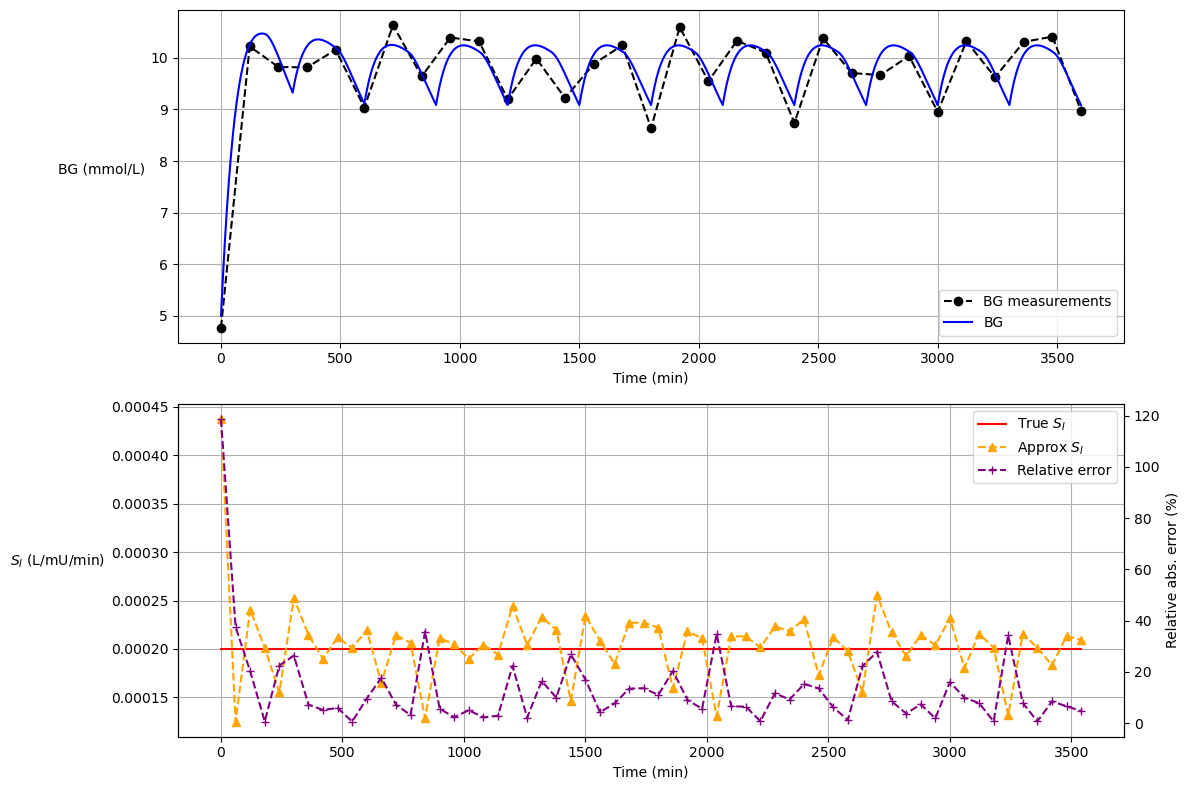
\includegraphics[width=0.9\linewidth]{figures/2_3.png}
    \caption[Caption for LOF]{Fitting the insulin sensitivity $S_I$ hourly using the integral-based parameter identification method on a patient model\footnotemark.}
    \label{fig:background}
\end{figure}

\footnotetext{The initial conditions of the patient model are $BG = 5.0$ (mmol/L), $I = 15.0$ (mU/L), $Q = 15.0$ (mU/L), $P1 = P2 = 0.0$ (mmol), with no external nutrition given. Measurements are sampled with additive Gaussian noise $r_k \sim N(0,0.25^2)$.}

\section{Summary}
% \sweExpl{Sammanfattning}
% \sweExpl{Det är trevligt om detta kapitel
%   avslutas med en sammanfattning. Till exempel kan du inkludera en tabell som
%   sammanfattar andras idéer och fördelar och nackdelar med varje - så som
%   senare kan du jämföra din lösning till var och en av dessa. Detta kommer
%   också att hjälpa dig att definiera de variabler som du kommer att använda
%   för din utvärdering.}

% \engExpl{It is nice to have this chapter conclude with a summary. For
%   example, you can include a table that summarizes other people's ideas and
%   benefits and drawbacks with each - so as later you can compare your solution
%   to each of them. This will also help you define the variables that you will
%   use for your evaluation.}

The Intensive Control Insulin-Nutrition-Glucose model provides a foundation to model glucose removal, insulin pharmacokinetics, and gastric absorption of glucose for tight glucose control in critically ill patients. Often, clinicians solely rely on blood glucose measurements, which limits the knowledge of the insulin-glucose dynamics in real-time. Utilizing nonlinear state estimators, such as the extended Kalman filter and the bootstrap particle filter, allow for estimation of all dynamics over time. To evaluate patient-specific parameters, model identifiability is used to make inferences about the parameters of interest. The current method of integral-based parameter identification is formulated with strict assumptions of blood glucose measurements, which limits the ability for clinicians to infer the health of the patient from the approximated patient-specific parameters. More in-depth methods can improve model identifiability for glucoregulation in critically ill patients.

\cleardoublepage
\chapter{Method or Methods}
\label{ch:methods}
\sweExpl{Metod eller Metodval}
\generalExpl{This chapter is about Engineering-related
  content, Methodologies and Methods.  Use a self-explaining title.\\The
  contents and structure of this chapter will change with your choice of
  methodology and methods.}



\generalExpl{Describe the engineering-related contents (preferably with models) and the research methodology and methods that are used in the degree project.\\
Give a theoretical description of the scientific or engineering methodology  you are going to use and why have you chosen this method. What other methods did you consider and why did you reject them.\\
In this chapter, you describe what engineering-related and scientific skills you are going to apply, such as modeling, analyzing, developing, and evaluating engineering-related and scientific content. The choice of these methods should be appropriate for the problem . Additionally, you should be consciousness of aspects relating to society and ethics (if applicable). The choices should also reflect your goals and what you (or someone else) should be able to do as a result of your solution - which could not be done well before you started.}

The purpose of this chapter is to provide an overview of the research method
used in this thesis. Section~\ref{sec:researchProcess} describes the research
process. Section~\ref{sec:researchParadigm} details the research
paradigm. Section~\ref{sec:dataCollection} focuses on the data collection
techniques used for this research. Section~\ref{sec:experimentalDesign}
describes the experimental design. Section~\ref{sec:assessingReliability}
explains the techniques used to evaluate the reliability and validity of the
data collected. Section~\ref{sec:plannedDataAnalysis} describes the method
used for the data analysis. Finally, Section~\ref{sec:evaluationFramework}
describes the framework selected to evaluate xxx.

\sweExpl{Vilka vetenskaplig eller ingenjörs-metodik ska du använda och varför har du valt den här metoden. Vilka andra metoder gjorde du övervägde du och varför du avvisar dem.
Vad är dina mål? (Vad ska du kunna göra som ett resultat av din lösning - vilken inte kan göras i god tid innan du började)
Vad du ska göra? Hur? Varför? Till exempel, om du har implementerat en artefakt vad gjorde du och varför? Hur kommer du utvärdera den.
Syftet med detta kapitel är att ge en översikt över forsknings metod som
används i denna avhandling. Avsnitt~\ref{sec:researchProcess} beskriver forskningsprocessen. Avsnitt~\ref{sec:researchParadigm} beskriver forskningsparadigmen detaljerat. Avsnitt~\ref{sec:dataCollection} fokuserar på datainsamlingstekniker som används för denna forskning. Avsnitt~\ref{sec:experimentalDesign} beskriver experimentell
design. Avsnitt~\ref{sec:assessingReliability} förklarar de tekniker som används för att utvärdera
tillförlitligheten och giltigheten av de insamlade uppgifterna. Avsnitt~\ref{sec:plannedDataAnalysis}
beskriver den metod som används för dataanalysen. Slutligen, Avsnitt~\ref{sec:evaluationFramework}
beskriver ramverket som valts för att utvärdera xxx.\\
Ofta kan man koppla ett antal följdfrågor till undersökningsfrågan och problemlösningen t ex\\
(1) Vilken process skall användas för konstruktion av lösningen och vilken process skall kopplas till denna för att svara på undersökningsfrågan?\\
(2) Hur och vilket resultat (storheter) skall presenteras både för att redovisa svar på undersökningsfrågan (resultatkapitlet i denna rapport) och redovisa resultat av problemlösningen (prototypen, ofta dokument som bilagor men vilka dokument och varför?).\\
(3) Vilken teori/teknik skall väljas och användas både för undersökningen (taxonomi, matematik, grafer, storheter mm)  och  problemlösning (UML, UseCases, Java mm) och varför?\\
(4) Vad behöver du som student leverera för att uppnå hög kvaliet (minimikrav) eller mycket hög kvalitet på examensarbetet?\\
(5) Frågorna kopplar till de följande underkapitlen.\\
(6) Resonemanget bygger på att studenter på hing-programmet ofta skall konstruera något åt problemägaren och att man till detta måste koppla en intressant ingenjörsfråga. Det finns hela tiden en dualism mellan dessa aspekter i exjobbet.
}

\section{Research Process}
\label{sec:researchProcess}

\sweExpl{Undersökningsrocess och utvecklingsprocess}

Figure~\ref{fig:researchprocess} shows the steps conducted in order to carry out this research. 

\sweExpl{Figur~\ref{fig:researchprocess} visar de steg som utförs för att genomföra\\
Beskriv, gärna med ett aktivitetsdiagram (UML?), din undersökningsprocess och utvecklingsprocess.  Du måste koppla ihop det akademiska intresset (undersökningsprocess) med ursprungsproblemet (utvecklingsprocess)
denna forskning.\\
Aktivitetsdiagram från t ex UML-standard}


 
\begin{figure}[!ht]
  \begin{center}
    
\includegraphics[width=0.5\textwidth]{figures/researchprocess.png}
  \end{center}
  \caption{Research Process}
  \label{fig:researchprocess}
\end{figure}

\generalExpl{Example of using customize item labels.}
Some steps in the process:
\begin{enumerate}[leftmargin=*, label=\textbf{Step \arabic*}, ref=Step \arabic*] %labelindent=1em for indent
    \itemsep0em
    \item \label{x:s1} plan experiment,
    \item \label{x:s2} conduct experiment,
    \item \label{x:s3} analyze data from the experiment, and
    \item \label{x:s4} discuss the results of the analysis.
\end{enumerate}

\sweExpl{Forskningsprocessen}


\section{Research Paradigm}
\label{sec:researchParadigm}
\sweExpl{Undersökningsparadigm\\
Exempelvis\\
Positivistisk (vad/hur fungerar det?) kvalitativ fallstudie med en deduktivt (förbestämd) vald ansats och ett induktivt(efterhand uppstår dataområden och data) insamlade av data och erfarenheter.}


\section{Data Collection}
\label{sec:dataCollection}
\sweExpl{Datainsamling\\
(Detta bör också visa att du är medveten om de sociala och etiska frågor som
kan vara relevanta för dina data insamlingsmetod.)}
\generalExpl{This should also show that you are aware of the social and ethical concerns that might be relevant to your data collection method.}



\subsection{Sampling}
\sweExpl{Stickprovsundersökning}

\subsection{Sample Size}
\sweExpl{Provstorleken}

\subsection{Target Population}
\sweExpl{Målgruppen}

\section[Experimental design/Planned Measurements]{Experimental design and\\Planned Measurements}
\label{sec:experimentalDesign}
\sweExpl{Experimentdesign/Mätuppställning}

\subsection{Test environment/test bed/model}
\engExpl{Describe everything that someone else would need to reproduce your test environment/test bed/model/… .}
\sweExpl{Testmiljö/testbädd/modell\\
Beskriv allt att någon annan skulle behöva återskapa din testmiljö / testbädd / modell / …}

\subsection{Hardware/Software to be used}
\sweExpl{Hårdvara / programvara som ska användas}


\section{Assessing reliability and validity of the data collected}
\label{sec:assessingReliability}
\sweExpl{Bedömning av validitet och reliabilitet hos använda metoder och insamlade data }


\subsection{Validity of method}
\label{sec:validtyOfMethod}
\sweExpl{Giltigheten av metoder\\
  Har dina metoder gett dig de rätta svaren och lösningarna? Var metoderna korrekta?}

\engExpl{How will you know if your results are valid?}
\engExpl{Remember that validity is about the \textit{accuracy} of a measurement while reliability is about the \textit{consistency} of the measurement values under the same conditions (\ie repeatability).}

\subsection{Reliability of method}
\label{sec:reliabilityOfMethod}
\sweExpl{Tillförlitlighet av för metoder\\
Hur bra är dina metoder, finns det bättre metoder? Hur kan du förbättra dem?}
\engExpl{How will you know if your results are reliable?}

\subsection{Data validity}
\label{sec:dataValidity}
\sweExpl{Giltigheten av uppgifter\\
Hur vet du om dina resultat är giltiga? Är ditt resultat rättvisande?}

\subsection{Reliability of data}
\label{sec:reliabilityOfData}
\sweExpl{Tillförlitlighet av data\\
Hur vet du om dina resultat är tillförlitliga? Hur bra är dina resultat?}


\section{Planned Data Analysis}
\label{sec:plannedDataAnalysis}
\sweExpl{Metod för analys av data}


\subsection{Data Analysis Technique}
\label{sec:dataAnalysisTechnique}
\sweExpl{Dataanalysteknik}

\subsection{Software Tools}
\label{sec:softwareTools}
\sweExpl{Mjukvaruverktyg}


\section{Evaluation framework}
\label{sec:evaluationFramework}
\sweExpl{Utvärdering och ramverk\\
Metod för utvärdering, jämförelse mm. Kopplar till kapitel~\ref{ch:resultsAndAnalysis}.}

\section{System documentation}
\label{sec:systemDocumentation}
\sweExpl{Systemdokumentation\\
Med vilka dokument och hur skall en konstruerad prototyp dokumenteras? Detta blir ofta bilagor till rapporten och det som problemägaren till det ursprungliga problemet (industrin) ofta vill ha.\\
Bland dessa bilagor återfinns ofta, och enligt någon angiven standard, kravdokument, arkitekturdokument, designdokumnet, implementationsdokument, driftsdokument, testprotokoll mm.}
\generalExpl{If this is going to be a complete document consider putting it in as an appendix, then just put the highlights here.}


\cleardoublepage
\chapter{What you did}\engExpl{Choose your own chapter title to describe this}
\label{ch:whatYouDid}
\sweExpl{[Vad gjorde du? Hur gick det till? – Välj lämplig rubrik (“Genomförande”, “Konstruktion”, ”Utveckling”  eller annat]}


\engExpl{What have you done? How did you do it? What design decisions did you make? How did what you did help you to meet your goals?}
\sweExpl{Vad du har gjort? Hur gjorde du det? Vilka designval gjorde du?\\
Hur kom det du hjälpte dig att uppnå dina mål?}

% the following sets the TOC entry to break after the & - note you have to include the first letter of the following word as it get swolled by the \texorpdfstring{}{} processing
\section[Hardware/Software design …/Model/Simulation model \&\texorpdfstring{\\}{ p} parameters/…]{Hardware/Software design …/Model/Simulation model \& parameters/…}
\sweExpl{Hårdvara / Mjukvarudesign ... / modell / Simuleringsmodell och parametrar / …}

Figure~\ref{fig:homepageicon} shows a simple icon for a home page. The time
to access this page when served will be quantified in a series of
experiments. The configurations that have been tested in the test bed are
listed in Table~\ref{tab:configstested}. In \SI{7.0}{\percent} of cases there was an error indicating xxxxx.

\sweExpl{Figur~\ref{fig:homepageicon}  visar en enkel ikon för en hemsida. Tiden för att få tillgång till den här sidan när den laddas kommer att kvantifieras i en serie experiment. De konfigurationer som har testats i provbänk listas ini tabell~\ref{tab:configstested}.\\
Vad du har gjort? Hur gjorde du det? Vilka designval gjorde du?}
 
\begin{figure}[!ht]
  \begin{center}
    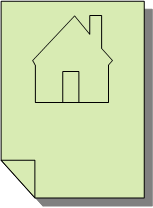
\includegraphics[width=0.25\textwidth]{figures/Homepage-icon.png}
  \end{center}
  \caption{Homepage icon}
  \label{fig:homepageicon}
\end{figure}

\begin{table}[!ht]
  \begin{center}
    \caption{Configurations tested}
    \label{tab:configstested}
    \resizebox{\columnwidth}{!}{%
    \begin{tabular}{l|c} % <-- Alignments: 1st column left, 2nd middle and 3rd right, with vertical lines in between
      \textbf{Configuration} & \textbf{Description} \\
      \hline
      1 & Simple test with one server\\
      2 & Simple test with one server\\
    \end{tabular}
    }
  \end{center}
\end{table}
\sweExpl{Testade konfigurationer}

\section{Implementation …/Modeling/Simulation/…}
\label{sec:implementationDetails}
\sweExpl{Implementering … / modellering / simulering / …}

Two commonly used simulators are:
\begin{description}[labelwidth =\widthof{\textbf{ns-2 or ns-3 simulator}}, leftmargin = !]
    \item[\textbf{Mininet}] This simulator uses traffic control (\texttt{tc}) to simulate network devices connected by links with specific bandwidth, packet loss rates, qdisc methods, etc.
    
    
    \item[\textbf{ns-2 or ns-3 simulator}] These simulators are very useful for simulating wireless communication links between moving devices. You can specific the mobility patterns of the nodes.
\end{description}

\subsection{Some examples of coding}
\engExpl{This section is simply to show some example of how you can include code in your thesis - this is not a section you would have in your thesis.}
\sweExpl{Det här avsnittet är helt enkelt för att visa ett exempel på hur du kan inkludera kod i ditt examensarbete - det här är inte ett avsnitt du skulle ha i ditt examensarbete.}

Listing~\ref{lst:helloWorldInC} shows an example of a simple program written
in C code.

\begin{lstlisting}[language={C}, caption={Hello world in C code}, label=lst:helloWorldInC]
int main() {
printf("hello, world");
return 0;
}
\end{lstlisting}


In contrast, Listing~\ref{lst:programmes} is an example of code in Python to
get a list of all of the programs at KTH.

\lstset{extendedchars=true}  %% This allows characters codes in the range 128-255
\begin{lstlisting}[language={Python}, caption={Using a python program to
    access the KTH API to get all of the programs at KTH}, label=lst:programmes]
KOPPSbaseUrl = 'https://www.kth.se'

def v1_get_programmes():
    global Verbose_Flag
    #
    # Use the KOPPS API to get the data
    # note that this returns XML
    url = "{0}/api/kopps/v1/programme".format(KOPPSbaseUrl)
    if Verbose_Flag:
        print("url: " + url)
    #
    r = requests.get(url)
    if Verbose_Flag:
        print("result of getting v1 programme: {}".format(r.text))
    #
    if r.status_code == requests.codes.ok:
        return r.text           # simply return the XML
    #
    return None
\end{lstlisting}
\FloatBarrier

\subsection{Some examples of figures in tikz}
\engExpl{This section is simply to show some example of how you can draw your own figures for in your thesis - this is not a section you would have in your thesis.}
\sweExpl{Det här avsnittet är helt enkelt för att visa ett exempel på hur du kan rita dina egna figurer i ditt examensarbete – det här är inte ett avsnitt du skulle ha i ditt examensarbete.}

These figures are just some examples to show that you can draw your own figures for in your thesis. This has two advantages: \first you do not have to worry about copyrights -- as these are your own figures and \Second the text is now readable and not simply a picture of text -- so screen readers can read the figure's contents to someone who is listening to the contents of your thesis.

\subsubsection{Azure's Form Recognizer}
\Cref{fig:processAnInvoice} shows the processing of key-value extraction from a PDF document using Azure's Form Recognizer. 

\tikzstyle{processBox} = [rectangle, rounded corners, minimum width=3cm, minimum height=1cm,text centered, draw=black, fill=red!20]
\tikzstyle{largeBox} = [rectangle, rounded corners, minimum width=3cm, minimum height=4cm,text centered, draw=black]
\begin{figure}[!ht]
\resizebox{1.1\textwidth}{!}{%
\begin{tikzpicture}
[align=left,node distance=2cm]

\node (document) [tape,tape bend top=none,draw,font=\sffamily] {PDF\\Document};
\node (GDM) [processBox,  right=0.5cm of document] {OCR};
\node (OCRoutput) [largeBox, right=1cm of GDM] {OCR output};

\node (kvp) [tape,tape bend top=none,draw,font=\sffamily, below=0.25cm of OCRoutput.north] {key-value\\pairs};
\node (entities) [tape,tape bend top=none,draw,font=\sffamily, above=0.35cm of OCRoutput.south] {Entities};
\node (Manual) [processBox, right=1cm of kvp] {Analyze the extracted\\key-value pairs};
\draw [-latex](document) --  (GDM);
\draw [-latex](kvp) --  (Manual);
\path[ draw
     , -latex'] let \p1=(GDM.east), \p2=(kvp.west) in (GDM.east) -- +(0.25*\x2-0.25*\x1, \y1) -- +(0.5*\x2-0.5*\x1, \y2) -- (kvp.west);
\path[ draw
     , -latex'] let \p1=(GDM.east), \p2=(kvp.west), \p3=(entities.west) in (GDM.east) --  +(0.25*\x2-0.25*\x1, \y1) -- +(0.5*\x3-0.5*\x1, \y3) -- (entities.west);
\end{tikzpicture}
}
\caption{The processing of key-value extraction from a PDF document using Azure's Form Recognizer}
  \label{fig:processAnInvoice}
\end{figure}
\FloatBarrier
\subsubsection{Hyper-V with Containers}
 \Cref{fig:hyperVcontainers} shows how Hyper-V deals with containers.
 
\tikzstyle{container} = [rectangle, rounded corners, minimum width=2cm, minimum height=1cm,text centered, draw=black, fill=blue!20]
\tikzstyle{containerization} = [rectangle, rounded corners, minimum width=13.25cm, minimum height=1cm,text centered, draw=black, fill=blue!20]
\tikzstyle{hypervisor} = [rectangle, rounded corners, minimum width=13.25cm, minimum height=1cm,text centered, draw=black, fill=red!20]
\tikzstyle{os} = [rectangle, rounded corners, minimum width=13.25cm, minimum height=1cm,text centered, draw=black, fill=orange!20]
\tikzstyle{guestos} = [rectangle, rounded corners, minimum width=2cm, minimum height=1cm,text centered, draw=black, fill=orange!40]
\tikzstyle{infrastructure} = [rectangle, rounded corners, minimum width=13.25cm, minimum height=1cm,text centered, draw=black, fill=green!20]

\tikzstyle{hos} = [rectangle, rounded corners, minimum width=6cm, minimum height=1cm,text centered, draw=black, fill=orange!20]
\tikzstyle{kernel} = [rectangle, rounded corners, minimum width=6cm, minimum height=1cm,text centered, draw=black, fill=purple!20]
\tikzstyle{services} = [rectangle, rounded corners, minimum width=3cm, minimum height=1cm,text centered, draw=black, fill=pink!20]
\begin{figure}[ht!]
    \centering
\resizebox{1\textwidth}{!}{%
\begin{tikzpicture}
[align=center,node distance=2cm]

\node (Infrastructure) [infrastructure, text width=13cm, text centered] {Infrastructure};
\node (OS1) [hos, anchor=north west, align=left, above=1.5cm of Infrastructure.north west, anchor=north west, text width=6cm, text centered] {Host OS};

\node (OS2) [hos, anchor= west, align=left, right=0.5cm of OS1.east, text width=6cm, anchor= west, text centered] {Host OS};

\node (Kernel1) [kernel, anchor=north west, align=left, above=1.5cm of OS1.north east, anchor=north east, text width=3cm, text centered] {Kernel};

\node (Kernel2) [kernel, anchor=north west, align=left, above=1.5cm of OS2.north east, anchor=north east, text width=3cm, text centered] {Kernel};

\node (ServiceA) [container, anchor=east, above=1 cm of Kernel1.east, anchor=east] {Services};
\node (AppA) [container,  left=0.25cm of ServiceA] {App 1};

\node (ServiceB) [container, anchor=east, above=1 cm of Kernel2.east, anchor=east] {Services};
\node (AppB) [container,  left=0.25cm of ServiceB] {App 2};
%\node (AppC) [container,  right=0.25cm of AppB] {App 3};

\draw[black,thick,dashed] ($(OS2.north west)+(-0.3,3.75)$)  rectangle ($(OS2.south east)+(0.5,-0.3)$);
\node[text width=5cm, text=red, above=0.1cm of ServiceB] 
    {\textbf{Container}};

\draw[red,thick,dotted] ($(Kernel2.north west)+(-0.3,1.6)$)  rectangle ($(Kernel2.south east)+(0.3,-0.3)$);
\node[text width=5cm, text=black, above=0.8cm of ServiceB] 
    {\textbf{VM}};
\end{tikzpicture}
}
    \caption{Hyper-V with containers}
    \label{fig:hyperVcontainers}
\end{figure}
\FloatBarrier
\subsubsection{\glsfmtshort{VM} versus Containers}
\Cref{fg:vmsVersusContainers} shows a comparison of virtual machines (VMs) versus containers.

\begin{figure*}[ht!]
    \centering
    \begin{subfigure}[t]{0.5\textwidth}
        \centering
\resizebox{1\textwidth}{!}{%
\begin{tikzpicture}
[align=left,node distance=2cm]

\node (AppA) [container,align=left] {App 1};
\node (AppB) [container,  right=0.25cm of AppA] {App 2};
\node (AppC) [container,  right=0.25cm of AppB] {App 3};

\node (GosA) [guestos,align=left,  below=0.25cm of AppA.south west,anchor=north west] {Guest OS};
\node (GosB) [guestos,  right=0.25cm of GosA] {Guest OS};
\node (GosC) [guestos,  right=0.25cm of GosB] {Guest OS};

\draw [decoration={brace,amplitude=0.5em},decorate, ultra thick,gray, transform canvas={xshift = 0.5cm}]
       (AppC.north -| AppC.east) -- (GosC.south -| AppC.east);
\node[text width=5cm,  right=1cm of GosC.north east] 
    {\textbf{VMs}};

\node (Hypervisor) [hypervisor, anchor=north west, align=left, below=0.25cm of GosA.south west, anchor=north west, text width=13cm, text centered] {Hypervisor};

\node (OS) [os, anchor=north west, align=left, below=0.25cm of Hypervisor.south west, anchor=north west, text width=13cm, text centered] {Host OS};

\node (Infrastructure) [infrastructure, anchor=north west, align=left, below=0.25cm of OS.south west, anchor=north west, text width=13cm, text centered] {Infrastructure};


\end{tikzpicture}
}
        \caption{VM}
    \end{subfigure}%
    ~ 
    \begin{subfigure}[t]{0.5\textwidth}
        \centering
        \resizebox{1\textwidth}{!}{%
\begin{tikzpicture}
[align=left,node distance=2cm]

\node (AppA) [container,align=left] {App 1};
\node (AppB) [container,  right=0.25cm of AppA] {App 2};
\node (AppC) [container,  right=0.25cm of AppB] {App 3};
\node[text width=5cm,  right=0.25cm of AppC] 
    {\textbf{Apps running in Containers}};


\node (Containerization) [containerization, anchor=north west, align=left, below=0.25cm of AppA.south west, anchor=north west, text width=13cm, text centered] {Docker Engine};

\node (OS) [os, anchor=north west, align=left, below=0.25cm of Containerization.south west, anchor=north west, text width=13cm, text centered] {Host OS};

\node (Infrastructure) [infrastructure, anchor=north west, align=left, below=0.25cm of OS.south west, anchor=north west, text width=13cm, text centered] {Infrastructure};


\end{tikzpicture}
}
        \caption{Containers}
    \end{subfigure}
    \caption{Virtual machines (VMs) versus Containers}
    \label{fg:vmsVersusContainers}
\end{figure*}

\cleardoublepage
\chapter{Results and Analysis}
\label{ch:resultsAndAnalysis}
\sweExpl{svensk: Resultat och Analys}

\engExpl{Sometimes this is split into two chapters.\\Keep in mind: How you are going to evaluate what you have done? What are your metrics?\\Analysis of your data and proposed solution\\Does this meet the goals which you had when you started?}

In this chapter, we present the results and discuss them.

\sweExpl{I detta kapitel presenterar vi resultaten och diskutera dem.\\Ibland delas detta upp i två kapitel.\\Hur du ska utvärdera vad du har gjort? Vad är din statistik?\\Analys av data och föreslagen lösning\\Innebär detta att uppfyllelse av de mål som du hade när du började?}

\section{Major results}
\sweExpl{Huvudsakliga resultat}

Some statistics of the delay measurements are shown in Table~\ref{tab:delayMeasurements}.
The delay has been computed from the time the GET request is received until the response is sent.

\sweExpl{Lite statistik av fördröjningsmätningarna visas i Tabell~\ref{tab:delayMeasurements}. Förseningen har beräknats från den tidpunkt då begäran GET tas emot fram till svaret skickas.}

\begin{table}[!ht]
  \begin{center}
    \caption{Delay measurement statistics}
    \label{tab:delayMeasurements}
    \begin{tabular}{l|S[table-format=4.2]|S[table-format=3.2]} % <-- Alignments: 1st column left, 2nd middle and 3rd right, with vertical lines in between
      \textbf{Configuration} & \textbf{Average delay (ns)} & \textbf{Median delay (ns)}\\
      \hline
      1 & 467.35 & 450.10\\
      2 & 1687.5 & 901.23\\
    \end{tabular}
  \end{center}
\end{table}

Table \ref{tab:ping_results} shows the measurement of round trip times from four hosts to and from a server.
\begin{table}[ht!]
\caption[RTT for 4 hosts]{Result for the ping measurements of RTT for 4 hosts} 
\label{tab:ping_results}
\vspace{1em}
\centering
\begin{tabular}{l *{4}{S[table-format=2.3]}}
{} & \multicolumn{4}{c}{host to server RTT in ms} \\
\cmidrule{2-5}
Host & \multicolumn{1}{c}{min}  & \multicolumn{1}{c}{avg} & \multicolumn{1}{c}{max} & \multicolumn{1}{c}{mdev} \\
\midrule
h1 & 5.625 & 5.625 & 5.625 & 0.0 \\
h2 & 2.909 & 2.909 & 1.909 & 0.0 \\
h3 & 5.007 & 5.007 & 5.007 & 0.0 \\
h4 & 2.308 & 2.308 & 2.308 & 0.0 \\
\midrule
\end{tabular}
\end{table}
\FloatBarrier

\sweExpl{Fördröj mätstatistik}
\sweExpl{Konfiguration | Genomsnittlig fördröjning (ns) | Median fördröjning (ns)}

Figure \ref{fig:processing_vs_payload_length} shows an example of the performance as measured in the experiments.

\begin{figure}[!ht]
% GNUPLOT: LaTeX picture
\setlength{\unitlength}{0.240900pt}
\ifx\plotpoint\undefined\newsavebox{\plotpoint}\fi
\begin{picture}(1500,900)(0,0)
\sbox{\plotpoint}{\rule[-0.200pt]{0.400pt}{0.400pt}}%
\put(171.0,131.0){\rule[-0.200pt]{4.818pt}{0.400pt}}
\put(151,131){\makebox(0,0)[r]{ 1.5}}
\put(1419.0,131.0){\rule[-0.200pt]{4.818pt}{0.400pt}}
\put(171.0,212.0){\rule[-0.200pt]{4.818pt}{0.400pt}}
\put(151,212){\makebox(0,0)[r]{ 2}}
\put(1419.0,212.0){\rule[-0.200pt]{4.818pt}{0.400pt}}
\put(171.0,292.0){\rule[-0.200pt]{4.818pt}{0.400pt}}
\put(151,292){\makebox(0,0)[r]{ 2.5}}
\put(1419.0,292.0){\rule[-0.200pt]{4.818pt}{0.400pt}}
\put(171.0,373.0){\rule[-0.200pt]{4.818pt}{0.400pt}}
\put(151,373){\makebox(0,0)[r]{ 3}}
\put(1419.0,373.0){\rule[-0.200pt]{4.818pt}{0.400pt}}
\put(171.0,454.0){\rule[-0.200pt]{4.818pt}{0.400pt}}
\put(151,454){\makebox(0,0)[r]{ 3.5}}
\put(1419.0,454.0){\rule[-0.200pt]{4.818pt}{0.400pt}}
\put(171.0,534.0){\rule[-0.200pt]{4.818pt}{0.400pt}}
\put(151,534){\makebox(0,0)[r]{ 4}}
\put(1419.0,534.0){\rule[-0.200pt]{4.818pt}{0.400pt}}
\put(171.0,615.0){\rule[-0.200pt]{4.818pt}{0.400pt}}
\put(151,615){\makebox(0,0)[r]{ 4.5}}
\put(1419.0,615.0){\rule[-0.200pt]{4.818pt}{0.400pt}}
\put(171.0,695.0){\rule[-0.200pt]{4.818pt}{0.400pt}}
\put(151,695){\makebox(0,0)[r]{ 5}}
\put(1419.0,695.0){\rule[-0.200pt]{4.818pt}{0.400pt}}
\put(171.0,776.0){\rule[-0.200pt]{4.818pt}{0.400pt}}
\put(151,776){\makebox(0,0)[r]{ 5.5}}
\put(1419.0,776.0){\rule[-0.200pt]{4.818pt}{0.400pt}}
\put(171.0,131.0){\rule[-0.200pt]{0.400pt}{4.818pt}}
\put(171,90){\makebox(0,0){ 0}}
\put(171.0,756.0){\rule[-0.200pt]{0.400pt}{4.818pt}}
\put(298.0,131.0){\rule[-0.200pt]{0.400pt}{4.818pt}}
\put(298,90){\makebox(0,0){ 10}}
\put(298.0,756.0){\rule[-0.200pt]{0.400pt}{4.818pt}}
\put(425.0,131.0){\rule[-0.200pt]{0.400pt}{4.818pt}}
\put(425,90){\makebox(0,0){ 20}}
\put(425.0,756.0){\rule[-0.200pt]{0.400pt}{4.818pt}}
\put(551.0,131.0){\rule[-0.200pt]{0.400pt}{4.818pt}}
\put(551,90){\makebox(0,0){ 30}}
\put(551.0,756.0){\rule[-0.200pt]{0.400pt}{4.818pt}}
\put(678.0,131.0){\rule[-0.200pt]{0.400pt}{4.818pt}}
\put(678,90){\makebox(0,0){ 40}}
\put(678.0,756.0){\rule[-0.200pt]{0.400pt}{4.818pt}}
\put(805.0,131.0){\rule[-0.200pt]{0.400pt}{4.818pt}}
\put(805,90){\makebox(0,0){ 50}}
\put(805.0,756.0){\rule[-0.200pt]{0.400pt}{4.818pt}}
\put(932.0,131.0){\rule[-0.200pt]{0.400pt}{4.818pt}}
\put(932,90){\makebox(0,0){ 60}}
\put(932.0,756.0){\rule[-0.200pt]{0.400pt}{4.818pt}}
\put(1059.0,131.0){\rule[-0.200pt]{0.400pt}{4.818pt}}
\put(1059,90){\makebox(0,0){ 70}}
\put(1059.0,756.0){\rule[-0.200pt]{0.400pt}{4.818pt}}
\put(1185.0,131.0){\rule[-0.200pt]{0.400pt}{4.818pt}}
\put(1185,90){\makebox(0,0){ 80}}
\put(1185.0,756.0){\rule[-0.200pt]{0.400pt}{4.818pt}}
\put(1312.0,131.0){\rule[-0.200pt]{0.400pt}{4.818pt}}
\put(1312,90){\makebox(0,0){ 90}}
\put(1312.0,756.0){\rule[-0.200pt]{0.400pt}{4.818pt}}
\put(1439.0,131.0){\rule[-0.200pt]{0.400pt}{4.818pt}}
\put(1439,90){\makebox(0,0){ 100}}
\put(1439.0,756.0){\rule[-0.200pt]{0.400pt}{4.818pt}}
\put(171.0,131.0){\rule[-0.200pt]{0.400pt}{155.380pt}}
\put(171.0,131.0){\rule[-0.200pt]{305.461pt}{0.400pt}}
\put(1439.0,131.0){\rule[-0.200pt]{0.400pt}{155.380pt}}
\put(171.0,776.0){\rule[-0.200pt]{305.461pt}{0.400pt}}
\put(30,453){\rotatebox{-270}{\makebox(0,0){Processing time (ms)}}}
\put(805,29){\makebox(0,0){Payload size (bytes)}}
\put(868.0,131.0){\rule[-0.200pt]{0.400pt}{84.074pt}}
\put(995.0,131.0){\rule[-0.200pt]{0.400pt}{98.287pt}}
\put(1173.0,131.0){\rule[-0.200pt]{0.400pt}{118.041pt}}
\put(1325.0,131.0){\rule[-0.200pt]{0.400pt}{134.904pt}}
\put(1350.0,131.0){\rule[-0.200pt]{0.400pt}{137.795pt}}
\put(1439.0,131.0){\rule[-0.200pt]{0.400pt}{155.380pt}}
\end{picture}
\caption[A GNUplot figure]{Processing time vs. payload length}\vspace{0.5cm}
\label{fig:processing_vs_payload_length}
\end{figure}
\FloatBarrier		

Given these measurements, we can calculate our processing bit rate as the inverse of the time it takes to process an additional byte divided by 8 bits per byte:

\[
	\text{bit rate} = \frac{1}{\frac{\text{time}_{\text{byte}}}{8}} = 20.03 \quad kb/s
\] 

\Cref{tab:majorMarkupLMDetailedResult} shows another table in which some values have been set in bold (using \textbackslash B) to emphasize them. Note how the \texttt{S} formatting has been modified so that it considers the weight of the characters and this is able to decimal align even these hold faced numbers with the numbers in the column above them.

\begin{table}[!ht]
    \centering
    \caption{Median values of sandwich attributes}
    \label{tab:majorMarkupLMDetailedResult}
    \begin{tabular}{l *{2}{S[detect-weight,mode=text,table-format=3.2]}}
        & \multicolumn{2}{c}{\textbf{sites}}\\
        \cmidrule{2-3}
        \textbf{Attribute} & \textbf{A} & \textbf{B} \\
        \midrule
        price (in SEK) & 36.5 & 71.3 \\
        protean (g) & 97.2 & 100.0 \\
        salt (mg) & 9.7 & 9.3 \\
        \hline
        \textbf{Average customer rating in \%} & \B 82.2 & \B 89.9 \\
        \midrule
    \end{tabular}
\end{table}
\FloatBarrier

\section{Reliability Analysis}
\sweExpl{Analys av tillförlitlighet\\
Tillförlitlighet i metod och data}

\section{Validity Analysis}
\sweExpl{Analys av validitet\\
Validitet i metod och data}

\cleardoublepage
\chapter{Discussion}
\label{ch:discussion}
\sweExpl{Diskussion\\
Förbättringsförslag?}
\generalExpl{This can be a separate chapter or a section in the previous chapter.}

\cleardoublepage
\chapter{Conclusions and Future work}
\label{ch:conclusionsAndFutureWork}
\sweExpl{Slutsats och framtida arbete}

\generalExpl{Add text to introduce the subsections of this chapter.}

\section{Conclusions}
\label{sec:conclusions}
\sweExpl{Slutsatser}
\engExpl{Describe the conclusions (reflect on the whole introduction given in Chapter 1).}


  
\engExpl{Discuss the positive effects and the drawbacks.\\
Describe the evaluation of the results of the degree project.\\
Did you meet your goals?\\
What insights have you gained?\\
What suggestions can you give to others working in this area?\\
If you had it to do again, what would you have done differently?}

\sweExpl{Uppfyllde du dina mål?\\
Vilka insikter har du fått?\\
Vilka förslag kan du ge till andra som arbetar inom detta område?
Om du skulle göra detta igen, vad skulle du ha gjort annorlunda?}

\section{Limitations}
\label{sec:limitations}
\sweExpl{Begränsande faktorer\\Vad gjorde du som begränsade dina ansträngningar? Vilka är begränsningarna i dina resultat?}
\engExpl{What did you find that limited your efforts? What are the limitations of your results?}


\section{Future work}
\label{sec:futureWork}
\sweExpl{Vad du har kvar ogjort?\\Vad är nästa självklara saker som ska göras?\\Vad tips kan du ge till nästa person som kommer att följa upp på ditt arbete?}
\engExpl{Describe valid future work that you or someone else could or should do.\\
Consider: What you have left undone? What are the next obvious things to be done? What hints can you give to the next person who is going to follow up on your work?}



Due to the breadth of the problem, only some of the initial goals have been
met. In these section we will focus on some of the remaining issues that
should be addressed in future work. ...

\subsection{What has been left undone?}
\label{what-has-been-left-undone}

The prototype does not address the third requirment, \ie a yearly unavailability of less than 3 minutes, this remains an open problem. ...

\subsubsection{Cost analysis}
\generalExpl{Example of a missing component}
The current prototype works, but the performance from a cost perspective makes this an impractical solution. Future work must reduce the cost of this solution, to do so a cost analysis needs to first be done. ...

\subsubsection{Security}
\generalExpl{Example of a missing component}
A future research effort is needed to address the security holes that results from using a self-signed certificate. Page filling text mass. Page filling text mass. ...


\subsection{Next obvious things to be done}

In particular, the author of this thesis wishes to point out xxxxxx remains as a problem to be solved. Solving this problem is the next thing that should be done. ...

\section{Reflections}
\label{sec:reflections}
\sweExpl{Reflektioner}
\sweExpl{Vilka är de relevanta ekonomiska, sociala, miljömässiga och etiska aspekter av ditt arbete?}
\engExpl{What are the relevant economic, social,
  environmental, and ethical aspects of your work?
}



One of the most important results is the reduction in the amount of
energy required to process each packet while at the same time reducing the
time required to process each packet.

The thesis contributes to the \gls{UN}\enspace\glspl{SDG} numbers 1 and 9 by
xxxx. 




\noindent\rule{\textwidth}{0.4mm}
\engExpl{In the references, let Zotero or other tool fill this in for you. I suggest an extended version of the IEEE style, to include URLs, DOIs, ISBNs, etc., to make it easier for your reader to find them. This will make life easier for your opponents and examiner. \\IEEE Editorial Style Manual: \url{https://www.ieee.org/content/dam/ieee-org/ieee/web/org/conferences/style_references_manual.pdf}}
\sweExpl{Låt Zotero eller annat verktyg fylla i det här för dig. Jag föreslår en utökad version av IEEE stil - att inkludera webbadresser, DOI, ISBN etc. - för att göra det lättare för läsaren att hitta dem. Detta kommer att göra livet lättare för dina opponenter och examinator.}

\cleardoublepage
% Print the bibliography (and make it appear in the table of contents)
\renewcommand{\bibname}{References}
\addcontentsline{toc}{chapter}{References}

\ifbiblatex
    %\typeout{Biblatex current language is \currentlang}
    \printbibliography[heading=bibintoc]
\else
    \bibliography{references, myreferences}
\fi



% \warningExpl{If you do not have an appendix, do not include the \textbackslash cleardoublepage command below, otherwise the last page number in the meta data will be one too large.}
\cleardoublepage
\appendix
\renewcommand{\chaptermark}[1]{\markboth{Appendix \thechapter\relax:\thinspace\relax#1}{}}
\chapter{Something Extra}
\sweExpl{svensk: Extra Material som Bilaga}

\section{Just for testing KTH colors}
\ifdigitaloutput
    \textbf{You have selected to optimize for digital output}
\else
    \textbf{You have selected to optimize for print output}
\fi
\begin{itemize}[noitemsep]
    \item Primary color
    \begin{itemize}
    \item \textcolor{kth-blue}{kth-blue \ifdigitaloutput
    actually Deep sea
    \fi} {\color{kth-blue} \rule{0.3\linewidth}{1mm} }\\

    \item \textcolor{kth-blue80}{kth-blue80} {\color{kth-blue80} \rule{0.3\linewidth}{1mm} }\\
\end{itemize}

\item  Secondary colors
\begin{itemize}[noitemsep]
    \item \textcolor{kth-lightblue}{kth-lightblue \ifdigitaloutput
    actually Stratosphere
    \fi} {\color{kth-lightblue} \rule{0.3\linewidth}{1mm} }\\

    \item \textcolor{kth-lightred}{kth-lightred \ifdigitaloutput
    actually Fluorescence\fi} {\color{kth-lightred} \rule{0.3\linewidth}{1mm} }\\

    \item \textcolor{kth-lightred80}{kth-lightred80} {\color{kth-lightred80} \rule{0.3\linewidth}{1mm} }\\

    \item \textcolor{kth-lightgreen}{kth-lightgreen \ifdigitaloutput
    actually Front-lawn\fi} {\color{kth-lightgreen} \rule{0.3\linewidth}{1mm} }\\

    \item \textcolor{kth-coolgray}{kth-coolgray \ifdigitaloutput
    actually Office\fi} {\color{kth-coolgray} \rule{0.3\linewidth}{1mm} }\\

    \item \textcolor{kth-coolgray80}{kth-coolgray80} {\color{kth-coolgray80} \rule{0.3\linewidth}{1mm} }
\end{itemize}
\end{itemize}

\textcolor{black}{black} {\color{black} \rule{\linewidth}{1mm} }

% Include an example of using nomenclature
\ifnomenclature
\cleardoublepage
\chapter{Main equations}
\label{ch:NomenclatureExamples}
This appendix gives some examples of equations that are used throughout this thesis.
\section{A simple example}
The following example is adapted from Figure 1 of the documentation for the package nomencl (\url{https://ctan.org/pkg/nomencl}).
\begin{equation}\label{eq:mainEq}
a=\frac{N}{A}
\end{equation}
\nomenclature{$a$}{The number of angels per unit area\nomrefeq}%       %% include the equation number in the list
\nomenclature{$N$}{The number of angels per needle point\nomrefpage}%  %% include the page number in the list
\nomenclature{$A$}{The area of the needle point}%
The equation $\sigma = m a$%
\nomenclature{$\sigma$}{The total mass of angels per unit area\nomrefeqpage}%
\nomenclature{$m$}{The mass of one angel}
follows easily from \Cref{eq:mainEq}.

\section{An even simpler example}
The formula for the diameter of a circle is shown in \Cref{eq:secondEq} area of a circle is shown in \cref{eq:thirdEq}.
\begin{equation}\label{eq:secondEq}
D_{circle}=2\pi r
\end{equation}
\nomenclature{$D_{circle}$}{The diameter of a circle\nomrefeqpage}%
\nomenclature{$r$}{The radius of a circle\nomrefeqpage}%

\begin{equation}\label{eq:thirdEq}
A_{circle}=\pi r^2
\end{equation}
\nomenclature{$A_{circle}$}{The area of a circle\nomrefeqpage}%

Some more text that refers to \eqref{eq:thirdEq}.
\fi  %% end of nomenclature example

\cleardoublepage
% Information for authors
%\include{README_author}
% \subfile{README_author}

\cleardoublepage
% information about the template for everyone
% \input{README_notes/README_notes}

\begin{comment}
% information for examiners
\ifxeorlua
\cleardoublepage
\input{README_notes/README_examiner_notes}
\fi
\end{comment}

\begin{comment}
% information for administrators
\ifxeorlua
\cleardoublepage
\input{README_notes/README_for_administrators.tex}
\fi
\end{comment}

%% The following label is necessary for computing the last page number of the body of the report to include in the "For DIVA" information
\label{pg:lastPageofMainmatter}

\cleardoublepage
\clearpage\thispagestyle{empty}\mbox{} % empty page with backcover on the other side
\kthbackcover
\fancyhead{}  % Do not use header on this extra page or pages
\section*{€€€€ For DIVA €€€€}
\lstset{numbers=none} %% remove any list line numbering
\divainfo{pg:lastPageofPreface}{pg:lastPageofMainmatter}

% If there is an acronyms.tex file,
% add it to the end of the For DIVA information
% so that it can be used with the abstracts
\IfFileExists{lib/acronyms.tex}{
\section*{acronyms.tex}
\lstinputlisting[language={[LaTeX]TeX}, basicstyle=\ttfamily\color{black},
commentstyle=\color{black}, backgroundcolor=\color{white}]{lib/acronyms.tex}
}
{}

\end{document}